\chapter{Wstęp}
Dla prostoty i przejrzystości sprawozdania wykorzystane zostały oznaczenia pierwotnie wprowadzone w skrypcie z przedmiotu STP.

\bigskip

Zadane wartości:

\smallskip

$W1=50\%$

\smallskip

$G1_{\mathrm{pp}}=U_{\mathrm{pp}}=30$

\smallskip

$T=1s$ (okres próbkowania)

\bigskip

Ograniczenia:

\smallskip

$0 \le G1(k) \le 100$

\chapter{Podpunkt 1}
Sprawdzenie możliwości sterowania i pomiaru w komunikacji ze stanowiskiem odbyło się poprzez wysłanie do stanowiska kilku różnych wartości sterowania i zaobserwowanie odpowiedniej odpowiedzi stanowiska oraz zmian w napływających danych.

Pomiar wartości temperatury w punkcie pracy odbył się zgodnie z poleceniem poprzez zadanie wartości sygnałów $W1$, $G1$, a następnie zarejestrowanie wartości sygnału $T1$ po ustabilizowaniu się układu. Warto w tym momencie zauważyć, że początkowo układ bardzo silnie oscylował wokół punktu pracy oraz w bardzo niewielkim stopniu reagował na sterowanie, dopiero po kilkudziesięciu minutach od rozpoczęcia laboratorium udało się zidentyfikować jako przyczynę tego zachowania okno otwarte w bezpośrednim sąsiedztwie układu. Po zamknięciu okna temperatura zarejestrowana w punkcie pracy to $T1=\num{33,2}$.

Na rys. \ref{R1} przestawiono stabilizację układu w punkcie pracy.

\begin{figure}[ht]
\centering
% This file was created by matlab2tikz.
%
%The latest updates can be retrieved from
%  http://www.mathworks.com/matlabcentral/fileexchange/22022-matlab2tikz-matlab2tikz
%where you can also make suggestions and rate matlab2tikz.
%
\definecolor{mycolor1}{rgb}{0.00000,0.44700,0.74100}%
%
\begin{tikzpicture}

\begin{axis}[%
width=4.521in,
height=3.566in,
at={(0.758in,0.481in)},
scale only axis,
xmin=0,
xmax=250,
xtick={0,50,100,150,200,250},
xlabel style={font=\color{white!15!black}},
xlabel={k},
ymin=25,
ymax=40,
ytick={25,30,35,40},
ylabel style={font=\color{white!15!black}},
ylabel={y},
axis background/.style={fill=white}
]
\addplot [color=mycolor1, forget plot]
  table[row sep=crcr]{%
1	32.68\\
2	32.68\\
3	32.68\\
4	32.68\\
5	32.68\\
6	32.68\\
7	32.68\\
8	32.68\\
9	32.68\\
10	32.68\\
11	32.68\\
12	32.75\\
13	32.75\\
14	32.75\\
15	32.75\\
16	32.75\\
17	32.81\\
18	32.75\\
19	32.81\\
20	32.81\\
21	32.81\\
22	32.81\\
23	32.81\\
24	32.81\\
25	32.81\\
26	32.81\\
27	32.81\\
28	32.81\\
29	32.87\\
30	32.87\\
31	32.81\\
32	32.81\\
33	32.81\\
34	32.81\\
35	32.81\\
36	32.81\\
37	32.81\\
38	32.81\\
39	32.81\\
40	32.81\\
41	32.81\\
42	32.87\\
43	32.87\\
44	32.87\\
45	32.87\\
46	32.87\\
47	32.87\\
48	32.87\\
49	32.87\\
50	32.87\\
51	32.87\\
52	32.87\\
53	32.87\\
54	32.87\\
55	32.87\\
56	32.87\\
57	32.87\\
58	32.87\\
59	32.87\\
60	32.87\\
61	32.87\\
62	32.87\\
63	32.87\\
64	32.87\\
65	32.81\\
66	32.81\\
67	32.81\\
68	32.81\\
69	32.81\\
70	32.81\\
71	32.81\\
72	32.81\\
73	32.81\\
74	32.81\\
75	32.81\\
76	32.81\\
77	32.81\\
78	32.75\\
79	32.81\\
80	32.81\\
81	32.81\\
82	32.75\\
83	32.75\\
84	32.75\\
85	32.75\\
86	32.81\\
87	32.75\\
88	32.81\\
89	32.81\\
90	32.81\\
91	32.81\\
92	32.81\\
93	32.87\\
94	32.93\\
95	33\\
96	33.12\\
97	33.25\\
98	33.37\\
99	33.43\\
100	33.5\\
101	33.5\\
102	33.5\\
103	33.5\\
104	33.5\\
105	33.5\\
106	33.5\\
107	33.43\\
108	33.43\\
109	33.43\\
110	33.43\\
111	33.37\\
112	33.37\\
113	33.37\\
114	33.37\\
115	33.37\\
116	33.31\\
117	33.37\\
118	33.31\\
119	33.31\\
120	33.31\\
121	33.31\\
122	33.31\\
123	33.31\\
124	33.31\\
125	33.31\\
126	33.31\\
127	33.31\\
128	33.25\\
129	33.25\\
130	33.25\\
131	33.25\\
132	33.25\\
133	33.25\\
134	33.25\\
135	33.25\\
136	33.25\\
137	33.18\\
138	33.18\\
139	33.18\\
140	33.18\\
141	33.18\\
142	33.25\\
143	33.18\\
144	33.18\\
145	33.25\\
146	33.18\\
147	33.18\\
148	33.18\\
149	33.18\\
150	33.18\\
151	33.18\\
152	33.18\\
153	33.12\\
154	33.12\\
155	33.12\\
156	33.12\\
157	33.12\\
158	33.12\\
159	33.12\\
160	33.12\\
161	33.12\\
162	33.12\\
163	33.12\\
164	33.12\\
165	33.12\\
166	33.12\\
167	33.12\\
168	33.12\\
169	33.06\\
170	33.12\\
171	33.12\\
172	33.12\\
173	33.12\\
174	33.06\\
175	33.12\\
176	33.12\\
177	33.12\\
178	33.12\\
179	33.12\\
180	33.12\\
181	33.12\\
182	33.12\\
183	33.12\\
184	33.12\\
185	33.12\\
186	33.12\\
187	33.18\\
188	33.18\\
189	33.18\\
190	33.18\\
191	33.12\\
192	33.18\\
193	33.18\\
194	33.12\\
195	33.18\\
196	33.12\\
197	33.12\\
198	33.12\\
199	33.18\\
200	33.12\\
201	33.18\\
202	33.18\\
203	33.18\\
204	33.18\\
205	33.18\\
206	33.18\\
207	33.18\\
208	33.18\\
209	33.18\\
210	33.18\\
211	33.12\\
212	33.12\\
213	33.12\\
214	33.12\\
215	33.12\\
216	33.12\\
217	33.12\\
218	33.12\\
219	33.12\\
220	33.12\\
221	33.12\\
222	33.12\\
223	33.12\\
224	33.12\\
225	33.12\\
226	33.12\\
227	33.12\\
228	33.12\\
229	33.06\\
230	33.06\\
231	33.06\\
232	33.06\\
233	33.06\\
234	33.06\\
235	33.06\\
236	33.06\\
237	33\\
238	33\\
239	33\\
240	33\\
241	33\\
242	33\\
243	33\\
244	33\\
245	33.06\\
246	33.06\\
247	33.06\\
248	33.06\\
249	33.06\\
250	33.06\\
};
\end{axis}
\end{tikzpicture}%
\caption{Stabilizacja układu w punkcie pracy}
\label{R1}
\end{figure}

\chapter{Podpunkt 2}
Odpowiedzi skokowe toru zakłócenie-wyjście zbadane zostały dla trzech wartości skoku, zgodnie z zaleceniem wybrano wartości: $\triangle z = \{10, 20, 30\}$, w chwili $k=\num{41}$. Na rys. \ref{R1} zamieszczono wyznaczone odpowiedzi.

\begin{figure}[ht]
\centering
% This file was created by matlab2tikz.
%
%The latest updates can be retrieved from
%  http://www.mathworks.com/matlabcentral/fileexchange/22022-matlab2tikz-matlab2tikz
%where you can also make suggestions and rate matlab2tikz.
%
\definecolor{mycolor1}{rgb}{0.00000,0.44700,0.74100}%
\definecolor{mycolor2}{rgb}{0.85000,0.32500,0.09800}%
\definecolor{mycolor3}{rgb}{0.92900,0.69400,0.12500}%
%
\begin{tikzpicture}

\begin{axis}[%
width=4.521in,
height=3.566in,
at={(0.758in,0.481in)},
scale only axis,
xmin=0,
xmax=300,
xtick={0,50,100,150,200,250,300},
xlabel style={font=\color{white!15!black}},
xlabel={$k$},
ymin=33,
ymax=36.5,
ytick={33,33.5,34,34.5,35,35.5,36,36.5},
yticklabels={{33},{33,5},{34},{34,5},{35},{35,5},{36},{36,5}},
ylabel style={font=\color{white!15!black}},
ylabel={$s$},
axis background/.style={fill=white},
legend style={at={(0.621,0.171)}, anchor=south west, legend cell align=left, align=left, draw=white!15!black}
]
\addplot [color=mycolor1]
  table[row sep=crcr]{%
1	33.75\\
2	33.75\\
3	33.75\\
4	33.75\\
5	33.75\\
6	33.75\\
7	33.75\\
8	33.68\\
9	33.68\\
10	33.75\\
11	33.75\\
12	33.75\\
13	33.75\\
14	33.81\\
15	33.75\\
16	33.81\\
17	33.81\\
18	33.81\\
19	33.81\\
20	33.81\\
21	33.81\\
22	33.81\\
23	33.87\\
24	33.87\\
25	33.81\\
26	33.87\\
27	33.87\\
28	33.87\\
29	33.87\\
30	33.87\\
31	33.87\\
32	33.87\\
33	33.87\\
34	33.87\\
35	33.87\\
36	33.87\\
37	33.87\\
38	33.87\\
39	33.87\\
40	33.93\\
41	33.87\\
42	33.87\\
43	33.93\\
44	33.93\\
45	33.93\\
46	33.93\\
47	33.93\\
48	34\\
49	34\\
50	34\\
51	34\\
52	34\\
53	34\\
54	34\\
55	34\\
56	34\\
57	34\\
58	34.06\\
59	34.06\\
60	34.06\\
61	34.06\\
62	34.06\\
63	34.06\\
64	34.06\\
65	34.12\\
66	34.06\\
67	34.12\\
68	34.12\\
69	34.12\\
70	34.12\\
71	34.12\\
72	34.12\\
73	34.12\\
74	34.12\\
75	34.12\\
76	34.12\\
77	34.18\\
78	34.18\\
79	34.18\\
80	34.18\\
81	34.18\\
82	34.18\\
83	34.25\\
84	34.25\\
85	34.25\\
86	34.25\\
87	34.25\\
88	34.25\\
89	34.25\\
90	34.25\\
91	34.25\\
92	34.25\\
93	34.31\\
94	34.31\\
95	34.31\\
96	34.31\\
97	34.31\\
98	34.31\\
99	34.37\\
100	34.37\\
101	34.37\\
102	34.37\\
103	34.37\\
104	34.37\\
105	34.37\\
106	34.37\\
107	34.37\\
108	34.43\\
109	34.37\\
110	34.37\\
111	34.43\\
112	34.43\\
113	34.43\\
114	34.43\\
115	34.5\\
116	34.5\\
117	34.5\\
118	34.5\\
119	34.5\\
120	34.5\\
121	34.5\\
122	34.5\\
123	34.5\\
124	34.5\\
125	34.5\\
126	34.5\\
127	34.5\\
128	34.5\\
129	34.5\\
130	34.5\\
131	34.5\\
132	34.5\\
133	34.56\\
134	34.56\\
135	34.56\\
136	34.56\\
137	34.56\\
138	34.56\\
139	34.56\\
140	34.56\\
141	34.56\\
142	34.56\\
143	34.56\\
144	34.56\\
145	34.56\\
146	34.56\\
147	34.56\\
148	34.56\\
149	34.56\\
150	34.56\\
151	34.5\\
152	34.5\\
153	34.5\\
154	34.5\\
155	34.5\\
156	34.5\\
157	34.56\\
158	34.5\\
159	34.56\\
160	34.56\\
161	34.56\\
162	34.56\\
163	34.56\\
164	34.56\\
165	34.56\\
166	34.56\\
167	34.56\\
168	34.56\\
169	34.56\\
170	34.56\\
171	34.62\\
172	34.62\\
173	34.56\\
174	34.62\\
175	34.56\\
176	34.56\\
177	34.62\\
178	34.62\\
179	34.62\\
180	34.62\\
181	34.62\\
182	34.62\\
183	34.62\\
184	34.62\\
185	34.62\\
186	34.62\\
187	34.62\\
188	34.62\\
189	34.62\\
190	34.62\\
191	34.62\\
192	34.62\\
193	34.62\\
194	34.62\\
195	34.62\\
196	34.68\\
197	34.68\\
198	34.68\\
199	34.62\\
200	34.62\\
201	34.62\\
202	34.62\\
203	34.62\\
204	34.62\\
205	34.62\\
206	34.62\\
207	34.62\\
208	34.62\\
209	34.62\\
210	34.62\\
211	34.56\\
212	34.62\\
213	34.62\\
214	34.62\\
215	34.62\\
216	34.56\\
217	34.62\\
218	34.62\\
219	34.62\\
220	34.62\\
221	34.62\\
222	34.68\\
223	34.68\\
224	34.68\\
225	34.68\\
226	34.68\\
227	34.68\\
228	34.75\\
229	34.75\\
230	34.68\\
231	34.75\\
232	34.75\\
233	34.75\\
234	34.75\\
235	34.75\\
236	34.75\\
237	34.75\\
238	34.81\\
239	34.81\\
240	34.81\\
241	34.81\\
242	34.81\\
243	34.75\\
244	34.75\\
245	34.75\\
246	34.75\\
247	34.75\\
248	34.75\\
249	34.75\\
250	34.75\\
251	34.75\\
252	34.75\\
253	34.75\\
254	34.75\\
255	34.75\\
256	34.75\\
257	34.75\\
258	34.75\\
259	34.75\\
260	34.75\\
261	34.75\\
262	34.75\\
263	34.75\\
264	34.68\\
265	34.68\\
266	34.68\\
267	34.68\\
268	34.68\\
269	34.68\\
270	34.68\\
271	34.68\\
272	34.68\\
273	34.75\\
274	34.68\\
275	34.75\\
276	34.68\\
277	34.68\\
278	34.68\\
279	34.68\\
280	34.68\\
281	34.68\\
282	34.68\\
283	34.68\\
284	34.68\\
285	34.68\\
286	34.68\\
287	34.68\\
288	34.68\\
289	34.68\\
290	34.68\\
291	34.68\\
292	34.68\\
293	34.68\\
294	34.68\\
295	34.68\\
296	34.68\\
297	34.68\\
298	34.68\\
299	34.68\\
300	34.75\\
};
\addlegendentry{$\triangle Z = 10$}

\addplot [color=mycolor2]
  table[row sep=crcr]{%
1	33.25\\
2	33.25\\
3	33.25\\
4	33.25\\
5	33.31\\
6	33.31\\
7	33.31\\
8	33.31\\
9	33.31\\
10	33.37\\
11	33.37\\
12	33.37\\
13	33.37\\
14	33.37\\
15	33.43\\
16	33.43\\
17	33.43\\
18	33.43\\
19	33.43\\
20	33.5\\
21	33.5\\
22	33.5\\
23	33.5\\
24	33.5\\
25	33.5\\
26	33.5\\
27	33.5\\
28	33.5\\
29	33.56\\
30	33.56\\
31	33.56\\
32	33.56\\
33	33.62\\
34	33.62\\
35	33.62\\
36	33.62\\
37	33.62\\
38	33.68\\
39	33.68\\
40	33.68\\
41	33.68\\
42	33.75\\
43	33.75\\
44	33.81\\
45	33.81\\
46	33.81\\
47	33.87\\
48	33.87\\
49	33.93\\
50	33.93\\
51	33.93\\
52	33.93\\
53	34\\
54	34\\
55	34\\
56	34.06\\
57	34.06\\
58	34.12\\
59	34.12\\
60	34.18\\
61	34.12\\
62	34.18\\
63	34.25\\
64	34.25\\
65	34.25\\
66	34.25\\
67	34.31\\
68	34.31\\
69	34.31\\
70	34.37\\
71	34.37\\
72	34.37\\
73	34.37\\
74	34.43\\
75	34.43\\
76	34.43\\
77	34.43\\
78	34.5\\
79	34.5\\
80	34.56\\
81	34.5\\
82	34.56\\
83	34.56\\
84	34.62\\
85	34.62\\
86	34.62\\
87	34.62\\
88	34.62\\
89	34.62\\
90	34.62\\
91	34.68\\
92	34.68\\
93	34.68\\
94	34.68\\
95	34.75\\
96	34.75\\
97	34.75\\
98	34.81\\
99	34.81\\
100	34.81\\
101	34.87\\
102	34.87\\
103	34.87\\
104	34.87\\
105	34.93\\
106	34.93\\
107	34.93\\
108	34.93\\
109	34.93\\
110	35\\
111	35\\
112	35\\
113	35\\
114	35\\
115	35\\
116	35\\
117	35\\
118	35.06\\
119	35.06\\
120	35.06\\
121	35.06\\
122	35.06\\
123	35.06\\
124	35.06\\
125	35.06\\
126	35.12\\
127	35.12\\
128	35.06\\
129	35.12\\
130	35.12\\
131	35.06\\
132	35.12\\
133	35.12\\
134	35.12\\
135	35.12\\
136	35.12\\
137	35.12\\
138	35.12\\
139	35.12\\
140	35.12\\
141	35.18\\
142	35.18\\
143	35.18\\
144	35.18\\
145	35.18\\
146	35.18\\
147	35.18\\
148	35.18\\
149	35.18\\
150	35.25\\
151	35.25\\
152	35.25\\
153	35.25\\
154	35.18\\
155	35.18\\
156	35.25\\
157	35.25\\
158	35.25\\
159	35.25\\
160	35.25\\
161	35.25\\
162	35.25\\
163	35.25\\
164	35.25\\
165	35.18\\
166	35.18\\
167	35.25\\
168	35.18\\
169	35.18\\
170	35.18\\
171	35.18\\
172	35.18\\
173	35.18\\
174	35.18\\
175	35.18\\
176	35.18\\
177	35.18\\
178	35.18\\
179	35.18\\
180	35.18\\
181	35.18\\
182	35.18\\
183	35.18\\
184	35.18\\
185	35.12\\
186	35.18\\
187	35.12\\
188	35.18\\
189	35.18\\
190	35.18\\
191	35.18\\
192	35.18\\
193	35.18\\
194	35.18\\
195	35.18\\
196	35.18\\
197	35.18\\
198	35.18\\
199	35.18\\
200	35.18\\
201	35.18\\
202	35.25\\
203	35.25\\
204	35.18\\
205	35.18\\
206	35.18\\
207	35.18\\
208	35.12\\
209	35.12\\
210	35.12\\
211	35.12\\
212	35.18\\
213	35.18\\
214	35.18\\
215	35.18\\
216	35.18\\
217	35.18\\
218	35.18\\
219	35.18\\
220	35.18\\
221	35.18\\
222	35.25\\
223	35.25\\
224	35.18\\
225	35.25\\
226	35.25\\
227	35.25\\
228	35.25\\
229	35.25\\
230	35.31\\
231	35.31\\
232	35.31\\
233	35.31\\
234	35.31\\
235	35.31\\
236	35.31\\
237	35.31\\
238	35.31\\
239	35.31\\
240	35.31\\
241	35.31\\
242	35.31\\
243	35.31\\
244	35.31\\
245	35.31\\
246	35.31\\
247	35.31\\
248	35.31\\
249	35.31\\
250	35.31\\
251	35.31\\
252	35.31\\
253	35.25\\
254	35.25\\
255	35.25\\
256	35.25\\
257	35.25\\
258	35.31\\
259	35.25\\
260	35.25\\
261	35.25\\
262	35.25\\
263	35.31\\
264	35.31\\
265	35.31\\
266	35.31\\
267	35.31\\
268	35.37\\
269	35.37\\
270	35.37\\
271	35.31\\
272	35.31\\
273	35.31\\
274	35.31\\
275	35.37\\
276	35.31\\
277	35.31\\
278	35.31\\
279	35.31\\
280	35.31\\
281	35.31\\
282	35.31\\
283	35.37\\
284	35.37\\
285	35.37\\
286	35.37\\
287	35.43\\
288	35.37\\
289	35.37\\
290	35.43\\
291	35.43\\
292	35.43\\
293	35.43\\
294	35.37\\
295	35.37\\
296	35.37\\
297	35.37\\
298	35.37\\
299	35.37\\
300	35.37\\
};
\addlegendentry{$\triangle Z = 20$}

\addplot [color=mycolor3]
  table[row sep=crcr]{%
1	33.25\\
2	33.25\\
3	33.25\\
4	33.25\\
5	33.25\\
6	33.25\\
7	33.25\\
8	33.25\\
9	33.25\\
10	33.25\\
11	33.25\\
12	33.25\\
13	33.31\\
14	33.31\\
15	33.31\\
16	33.31\\
17	33.37\\
18	33.37\\
19	33.37\\
20	33.43\\
21	33.43\\
22	33.43\\
23	33.43\\
24	33.5\\
25	33.5\\
26	33.5\\
27	33.56\\
28	33.56\\
29	33.56\\
30	33.62\\
31	33.62\\
32	33.62\\
33	33.68\\
34	33.68\\
35	33.75\\
36	33.75\\
37	33.75\\
38	33.81\\
39	33.81\\
40	33.87\\
41	33.87\\
42	33.93\\
43	33.93\\
44	33.93\\
45	34\\
46	34.06\\
47	34.06\\
48	34.12\\
49	34.12\\
50	34.12\\
51	34.18\\
52	34.18\\
53	34.18\\
54	34.25\\
55	34.25\\
56	34.31\\
57	34.31\\
58	34.37\\
59	34.37\\
60	34.37\\
61	34.37\\
62	34.43\\
63	34.43\\
64	34.43\\
65	34.43\\
66	34.5\\
67	34.5\\
68	34.5\\
69	34.5\\
70	34.56\\
71	34.56\\
72	34.56\\
73	34.62\\
74	34.62\\
75	34.62\\
76	34.68\\
77	34.68\\
78	34.68\\
79	34.75\\
80	34.75\\
81	34.81\\
82	34.81\\
83	34.81\\
84	34.81\\
85	34.87\\
86	34.87\\
87	34.87\\
88	34.93\\
89	34.93\\
90	34.93\\
91	34.93\\
92	35\\
93	35\\
94	35\\
95	35\\
96	35.06\\
97	35.06\\
98	35.12\\
99	35.06\\
100	35.12\\
101	35.12\\
102	35.12\\
103	35.18\\
104	35.18\\
105	35.18\\
106	35.18\\
107	35.18\\
108	35.18\\
109	35.18\\
110	35.25\\
111	35.25\\
112	35.25\\
113	35.25\\
114	35.25\\
115	35.25\\
116	35.31\\
117	35.31\\
118	35.31\\
119	35.31\\
120	35.31\\
121	35.37\\
122	35.37\\
123	35.37\\
124	35.37\\
125	35.37\\
126	35.37\\
127	35.37\\
128	35.43\\
129	35.43\\
130	35.43\\
131	35.43\\
132	35.43\\
133	35.43\\
134	35.43\\
135	35.43\\
136	35.43\\
137	35.43\\
138	35.43\\
139	35.5\\
140	35.5\\
141	35.5\\
142	35.5\\
143	35.43\\
144	35.5\\
145	35.43\\
146	35.5\\
147	35.5\\
148	35.5\\
149	35.5\\
150	35.5\\
151	35.56\\
152	35.56\\
153	35.56\\
154	35.56\\
155	35.56\\
156	35.56\\
157	35.56\\
158	35.56\\
159	35.56\\
160	35.56\\
161	35.56\\
162	35.56\\
163	35.62\\
164	35.62\\
165	35.62\\
166	35.56\\
167	35.62\\
168	35.62\\
169	35.62\\
170	35.62\\
171	35.62\\
172	35.62\\
173	35.62\\
174	35.62\\
175	35.68\\
176	35.68\\
177	35.68\\
178	35.68\\
179	35.68\\
180	35.68\\
181	35.68\\
182	35.68\\
183	35.75\\
184	35.75\\
185	35.75\\
186	35.75\\
187	35.75\\
188	35.75\\
189	35.75\\
190	35.75\\
191	35.81\\
192	35.81\\
193	35.81\\
194	35.81\\
195	35.81\\
196	35.81\\
197	35.81\\
198	35.81\\
199	35.81\\
200	35.81\\
201	35.81\\
202	35.81\\
203	35.81\\
204	35.81\\
205	35.81\\
206	35.81\\
207	35.81\\
208	35.81\\
209	35.81\\
210	35.81\\
211	35.81\\
212	35.81\\
213	35.81\\
214	35.81\\
215	35.81\\
216	35.81\\
217	35.81\\
218	35.81\\
219	35.75\\
220	35.75\\
221	35.75\\
222	35.75\\
223	35.75\\
224	35.75\\
225	35.81\\
226	35.81\\
227	35.81\\
228	35.81\\
229	35.81\\
230	35.81\\
231	35.81\\
232	35.81\\
233	35.81\\
234	35.75\\
235	35.81\\
236	35.75\\
237	35.75\\
238	35.75\\
239	35.81\\
240	35.81\\
241	35.81\\
242	35.81\\
243	35.81\\
244	35.81\\
245	35.81\\
246	35.75\\
247	35.81\\
248	35.81\\
249	35.81\\
250	35.81\\
251	35.81\\
252	35.87\\
253	35.87\\
254	35.87\\
255	35.87\\
256	35.87\\
257	35.87\\
258	35.87\\
259	35.93\\
260	35.93\\
261	35.93\\
262	35.93\\
263	36\\
264	36\\
265	36\\
266	36\\
267	36.06\\
268	36\\
269	36\\
270	36.06\\
271	36\\
272	36.06\\
273	36.06\\
274	36.06\\
275	36.06\\
276	36.06\\
277	36.06\\
278	36.06\\
279	36.06\\
280	36.06\\
281	36.06\\
282	36.12\\
283	36.06\\
284	36.06\\
285	36.12\\
286	36.12\\
287	36.12\\
288	36.12\\
289	36.12\\
290	36.12\\
291	36.12\\
292	36.06\\
293	36.12\\
294	36.12\\
295	36.12\\
296	36.12\\
297	36.12\\
298	36.12\\
299	36.12\\
300	36.12\\
};
\addlegendentry{$\triangle Z = 30$}

\end{axis}
\end{tikzpicture}%

\caption{Odpowiedź dla skoków zakłócenia z punktu pracy o $\triangle z = \{10, 20, 30\}$}
\label{R2}
\end{figure}

Różnice w wartościach przed wykonaniem samego skoku (które to powinny przyjmować wartość $U_{\mathrm{pp}}$) wynikają najprawdopodbniej z niedokładnego schłodzenia przez nas obiektu.

Obliczając wzmocnienie statyczne dla odpowiedzi skokowej na podstawie wzoru:
\begin{equation}
K=\frac{Y_{\mathrm{konc}}-Y_{\mathrm{pp}}}{\triangle U}
\end{equation}
dostajemy $K_{\mathrm{z}}=\num{0}$.

Wyznaczone wzmocnienia są TODO: Jakie? dla różnych skoków, warto też zauważyć, że temperatura ani przed skokiem, ani po stabilizacji nie przyjmuje stałej wartości, a jedynie oscyluje w ograniczonym przedziale. Wynikająca z wyboru punktu pracy oraz punktu stabilizacji niepewność wyznaczonych wzmocnień wynosi ok. $\pm \num{0,01}$ (wyznaczona jako różnica między wartościami skrajnymi).


\chapter{Podpunkt 3}
Na potrzeby algorytmu DMC pobrano i znormalizowano odpowiedzi skokowe dla obu torów sygnału. Skok sterowania wykonano z punktu pracy o $\triangle U = 10$, zaś skok zakłócenia z punktu pracy o $\triangle z = 30$. Do przekształcenia wykorzystany został wzór (\ref{step_norm}), zaś uzyskana odpowiedź skokowa została przedstawiona na rys. \ref{R3}. Kolejne wartości wyznaczonych odpowiedzi skokowych zadanego modelu zapisane są odpowiednio dla sterowania i zakłócenia w plikach \verb+step_response.txt+ oraz \verb+step_response2.txt+.
\begin{equation}
S_i = \frac{S_i^0 - Y_{\mathrm{pp}}}{\triangle U} \textrm{, dla } i=1,\ldots
\label{step_norm}
\end{equation}
\begin{equation}
S_i^{\mathrm{z}} = \frac{S_i^0 - Y_{\mathrm{pp}}}{\triangle z} \textrm{, dla } i=1,\ldots
\label{stepz_norm}
\end{equation}
gdzie $S_i^0$ to kolejne wartości dyskretnej odpowiedzi skokowej procesu dla danego toru, $\triangle U$ to wartość skoku sygnału sterującego (odpowiednio dla toru zakłócenia mamy $\triangle z$), zaś $S_i$ oraz $S_i^{\mathrm{z}}$ to kolejne wartości odpowiedzi skokowych odpowiednich torów wykorzystywane później przez algorytm DMC.

\begin{figure}[ht]
\centering
% This file was created by matlab2tikz.
%
%The latest updates can be retrieved from
%  http://www.mathworks.com/matlabcentral/fileexchange/22022-matlab2tikz-matlab2tikz
%where you can also make suggestions and rate matlab2tikz.
%
\definecolor{mycolor1}{rgb}{0.00000,0.44700,0.74100}%
\definecolor{mycolor2}{rgb}{0.85000,0.32500,0.09800}%
%
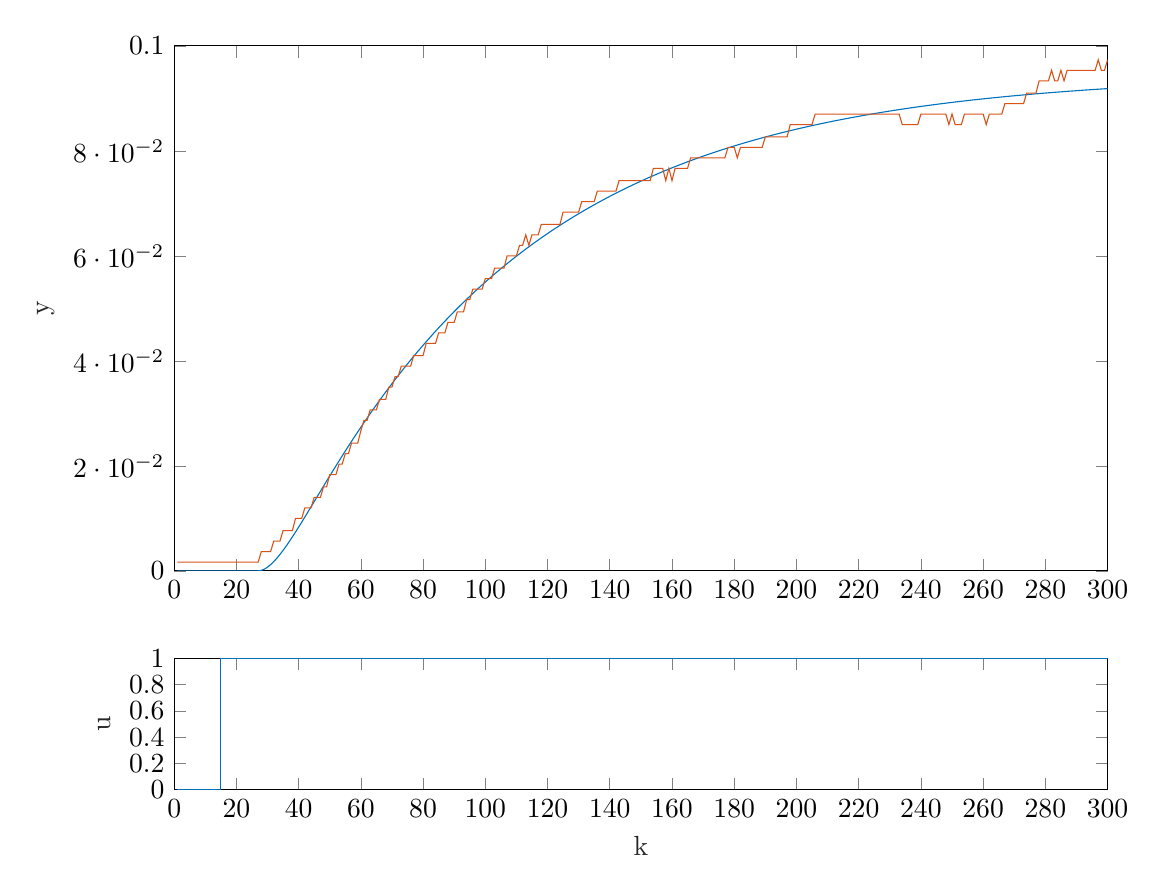
\begin{tikzpicture}

\begin{axis}[%
width=4.667in,
height=0.656in,
at={(0.583in,0.525in)},
scale only axis,
xmin=0,
xmax=300,
xlabel style={font=\color{white!15!black}},
xlabel={k},
ymin=0,
ymax=1,
ylabel style={font=\color{white!15!black}},
ylabel={u},
axis background/.style={fill=white}
]
\addplot[const plot, color=mycolor1, forget plot] table[row sep=crcr] {%
1	0\\
2	0\\
3	0\\
4	0\\
5	0\\
6	0\\
7	0\\
8	0\\
9	0\\
10	0\\
11	0\\
12	0\\
13	0\\
14	0\\
15	1\\
16	1\\
17	1\\
18	1\\
19	1\\
20	1\\
21	1\\
22	1\\
23	1\\
24	1\\
25	1\\
26	1\\
27	1\\
28	1\\
29	1\\
30	1\\
31	1\\
32	1\\
33	1\\
34	1\\
35	1\\
36	1\\
37	1\\
38	1\\
39	1\\
40	1\\
41	1\\
42	1\\
43	1\\
44	1\\
45	1\\
46	1\\
47	1\\
48	1\\
49	1\\
50	1\\
51	1\\
52	1\\
53	1\\
54	1\\
55	1\\
56	1\\
57	1\\
58	1\\
59	1\\
60	1\\
61	1\\
62	1\\
63	1\\
64	1\\
65	1\\
66	1\\
67	1\\
68	1\\
69	1\\
70	1\\
71	1\\
72	1\\
73	1\\
74	1\\
75	1\\
76	1\\
77	1\\
78	1\\
79	1\\
80	1\\
81	1\\
82	1\\
83	1\\
84	1\\
85	1\\
86	1\\
87	1\\
88	1\\
89	1\\
90	1\\
91	1\\
92	1\\
93	1\\
94	1\\
95	1\\
96	1\\
97	1\\
98	1\\
99	1\\
100	1\\
101	1\\
102	1\\
103	1\\
104	1\\
105	1\\
106	1\\
107	1\\
108	1\\
109	1\\
110	1\\
111	1\\
112	1\\
113	1\\
114	1\\
115	1\\
116	1\\
117	1\\
118	1\\
119	1\\
120	1\\
121	1\\
122	1\\
123	1\\
124	1\\
125	1\\
126	1\\
127	1\\
128	1\\
129	1\\
130	1\\
131	1\\
132	1\\
133	1\\
134	1\\
135	1\\
136	1\\
137	1\\
138	1\\
139	1\\
140	1\\
141	1\\
142	1\\
143	1\\
144	1\\
145	1\\
146	1\\
147	1\\
148	1\\
149	1\\
150	1\\
151	1\\
152	1\\
153	1\\
154	1\\
155	1\\
156	1\\
157	1\\
158	1\\
159	1\\
160	1\\
161	1\\
162	1\\
163	1\\
164	1\\
165	1\\
166	1\\
167	1\\
168	1\\
169	1\\
170	1\\
171	1\\
172	1\\
173	1\\
174	1\\
175	1\\
176	1\\
177	1\\
178	1\\
179	1\\
180	1\\
181	1\\
182	1\\
183	1\\
184	1\\
185	1\\
186	1\\
187	1\\
188	1\\
189	1\\
190	1\\
191	1\\
192	1\\
193	1\\
194	1\\
195	1\\
196	1\\
197	1\\
198	1\\
199	1\\
200	1\\
201	1\\
202	1\\
203	1\\
204	1\\
205	1\\
206	1\\
207	1\\
208	1\\
209	1\\
210	1\\
211	1\\
212	1\\
213	1\\
214	1\\
215	1\\
216	1\\
217	1\\
218	1\\
219	1\\
220	1\\
221	1\\
222	1\\
223	1\\
224	1\\
225	1\\
226	1\\
227	1\\
228	1\\
229	1\\
230	1\\
231	1\\
232	1\\
233	1\\
234	1\\
235	1\\
236	1\\
237	1\\
238	1\\
239	1\\
240	1\\
241	1\\
242	1\\
243	1\\
244	1\\
245	1\\
246	1\\
247	1\\
248	1\\
249	1\\
250	1\\
251	1\\
252	1\\
253	1\\
254	1\\
255	1\\
256	1\\
257	1\\
258	1\\
259	1\\
260	1\\
261	1\\
262	1\\
263	1\\
264	1\\
265	1\\
266	1\\
267	1\\
268	1\\
269	1\\
270	1\\
271	1\\
272	1\\
273	1\\
274	1\\
275	1\\
276	1\\
277	1\\
278	1\\
279	1\\
280	1\\
281	1\\
282	1\\
283	1\\
284	1\\
285	1\\
286	1\\
287	1\\
288	1\\
289	1\\
290	1\\
291	1\\
292	1\\
293	1\\
294	1\\
295	1\\
296	1\\
297	1\\
298	1\\
299	1\\
300	1\\
};
\end{axis}

\begin{axis}[%
width=4.667in,
height=2.625in,
at={(0.583in,1.619in)},
scale only axis,
xmin=0,
xmax=300,
ymin=0,
ymax=0.1,
ylabel style={font=\color{white!15!black}},
ylabel={y},
axis background/.style={fill=white}
]
\addplot [color=mycolor1, forget plot]
  table[row sep=crcr]{%
1	0\\
2	0\\
3	0\\
4	0\\
5	0\\
6	0\\
7	0\\
8	0\\
9	0\\
10	0\\
11	0\\
12	0\\
13	0\\
14	0\\
15	0\\
16	0\\
17	0\\
18	0\\
19	0\\
20	0\\
21	0\\
22	0\\
23	0\\
24	0\\
25	0\\
26	0\\
27	0\\
28	8.46657677711817e-05\\
29	0.000322071780209297\\
30	0.000689841089121847\\
31	0.00116858701633257\\
32	0.00174151698766157\\
33	0.00239408880822118\\
34	0.00311371243785129\\
35	0.00388949124424984\\
36	0.00471199750848349\\
37	0.00557307764918471\\
38	0.00646568323182034\\
39	0.00738372435006904\\
40	0.00832194241808434\\
41	0.00927579980436696\\
42	0.0102413840780393\\
43	0.0112153249333729\\
44	0.0121947221144226\\
45	0.013177082883743\\
46	0.0141602677718793\\
47	0.0151424435115385\\
48	0.0161220422054254\\
49	0.0170977259026053\\
50	0.0180683558674683\\
51	0.0190329659201357\\
52	0.0199907393093591\\
53	0.0209409886503055\\
54	0.0218831385215087\\
55	0.0228167103689742\\
56	0.0237413094120124\\
57	0.0246566132858058\\
58	0.0255623621907898\\
59	0.026458350349357\\
60	0.0273444185968046\\
61	0.0282204479563495\\
62	0.0290863540679163\\
63	0.0299420823576492\\
64	0.0307876038500603\\
65	0.0316229115377151\\
66	0.0324480172346134\\
67	0.0332629488492058\\
68	0.0340677480214581\\
69	0.0348624680757399\\
70	0.0356471722476929\\
71	0.0364219321487762\\
72	0.0371868264369906\\
73	0.0379419396664522\\
74	0.0386873612921054\\
75	0.0394231848090034\\
76	0.0401495070083072\\
77	0.0408664273345173\\
78	0.0415740473305034\\
79	0.0422724701586747\\
80	0.0429618001881774\\
81	0.0436421426393456\\
82	0.0443136032777934\\
83	0.0449762881515422\\
84	0.0456303033654554\\
85	0.0462757548880085\\
86	0.0469127483860813\\
87	0.0475413890840327\\
88	0.0481617816438107\\
89	0.0487740300632828\\
90	0.0493782375903436\\
91	0.0499745066506819\\
92	0.0505629387873671\\
93	0.0511436346106634\\
94	0.0517166937566859\\
95	0.0522822148537017\\
96	0.052840295495034\\
97	0.053391032217667\\
98	0.0539345204857704\\
99	0.0544708546784639\\
100	0.0550001280812325\\
101	0.0555224328804851\\
102	0.0560378601608114\\
103	0.0565464999045552\\
104	0.0570484409933718\\
105	0.0575437712114802\\
106	0.0580325772503632\\
107	0.0585149447146958\\
108	0.0589909581293181\\
109	0.059460700947088\\
110	0.0599242555574745\\
111	0.0603817032957703\\
112	0.0608331244528183\\
113	0.0612785982851603\\
114	0.0617182030255316\\
115	0.0621520158936311\\
116	0.0625801131071103\\
117	0.063002569892729\\
118	0.0634194604976362\\
119	0.0638308582007363\\
120	0.0642368353241106\\
121	0.0646374632444644\\
122	0.0650328124045778\\
123	0.065422952324738\\
124	0.0658079516141371\\
125	0.06618787798222\\
126	0.0665627982499694\\
127	0.0669327783611184\\
128	0.0672978833932801\\
129	0.067658177568988\\
130	0.0680137242666394\\
131	0.0683645860313385\\
132	0.0687108245856332\\
133	0.0690525008401423\\
134	0.0693896749040713\\
135	0.0697224060956134\\
136	0.0700507529522348\\
137	0.0703747732408424\\
138	0.0706945239678338\\
139	0.0710100613890282\\
140	0.0713214410194786\\
141	0.0716287176431648\\
142	0.0719319453225683\\
143	0.0722311774081279\\
144	0.0725264665475781\\
145	0.0728178646951703\\
146	0.073105423120777\\
147	0.0733891924188815\\
148	0.0736692225174517\\
149	0.0739455626867015\\
150	0.0742182615477386\\
151	0.0744873670811016\\
152	0.0747529266351865\\
153	0.0750149869345638\\
154	0.0752735940881883\\
155	0.0755287935975013\\
156	0.0757806303644282\\
157	0.0760291486992707\\
158	0.0762743923284968\\
159	0.0765164044024289\\
160	0.0767552275028305\\
161	0.0769909036503947\\
162	0.0772234743121334\\
163	0.0774529804086707\\
164	0.0776794623214392\\
165	0.0779029598997837\\
166	0.0781235124679695\\
167	0.0783411588321005\\
168	0.0785559372869448\\
169	0.0787678856226718\\
170	0.0789770411314999\\
171	0.079183440614257\\
172	0.0793871203868547\\
173	0.0795881162866772\\
174	0.0797864636788866\\
175	0.0799821974626443\\
176	0.0801753520772511\\
177	0.0803659615082065\\
178	0.080554059293188\\
179	0.0807396785279518\\
180	0.0809228518721552\\
181	0.0811036115551036\\
182	0.0812819893814202\\
183	0.0814580167366426\\
184	0.0816317245927443\\
185	0.0818031435135843\\
186	0.0819723036602848\\
187	0.0821392347965378\\
188	0.0823039662938418\\
189	0.0824665271366701\\
190	0.0826269459275698\\
191	0.082785250892195\\
192	0.0829414698842727\\
193	0.0830956303905039\\
194	0.0832477595353995\\
195	0.083397884086053\\
196	0.0835460304568501\\
197	0.0836922247141164\\
198	0.0838364925807035\\
199	0.083978859440515\\
200	0.084119350342973\\
201	0.0842579900074254\\
202	0.0843948028274948\\
203	0.0845298128753713\\
204	0.0846630439060476\\
205	0.0847945193614986\\
206	0.0849242623748061\\
207	0.0850522957742291\\
208	0.0851786420872205\\
209	0.0853033235443906\\
210	0.0854263620834185\\
211	0.0855477793529124\\
212	0.0856675967162184\\
213	0.0857858352551794\\
214	0.0859025157738443\\
215	0.0860176588021289\\
216	0.0861312845994276\\
217	0.0862434131581787\\
218	0.0863540642073811\\
219	0.0864632572160667\\
220	0.086571011396725\\
221	0.0866773457086844\\
222	0.0867822788614474\\
223	0.0868858293179828\\
224	0.0869880152979745\\
225	0.0870888547810266\\
226	0.0871883655098277\\
227	0.0872865649932721\\
228	0.0873834705095408\\
229	0.0874790991091416\\
230	0.0875734676179089\\
231	0.0876665926399645\\
232	0.0877584905606387\\
233	0.087849177549354\\
234	0.087938669562469\\
235	0.0880269823460872\\
236	0.0881141314388265\\
237	0.0882001321745537\\
238	0.0882849996850824\\
239	0.0883687489028354\\
240	0.0884513945634722\\
241	0.0885329512084815\\
242	0.0886134331877401\\
243	0.0886928546620372\\
244	0.0887712296055668\\
245	0.0888485718083855\\
246	0.0889248948788399\\
247	0.0890002122459601\\
248	0.0890745371618228\\
249	0.0891478827038835\\
250	0.0892202617772767\\
251	0.089291687117087\\
252	0.0893621712905899\\
253	0.0894317266994626\\
254	0.0895003655819665\\
255	0.0895681000151004\\
256	0.0896349419167252\\
257	0.0897009030476614\\
258	0.0897659950137576\\
259	0.0898302292679334\\
260	0.0898936171121939\\
261	0.0899561696996187\\
262	0.0900178980363239\\
263	0.0900788129833991\\
264	0.0901389252588179\\
265	0.0901982454393242\\
266	0.0902567839622928\\
267	0.090314551127566\\
268	0.0903715570992659\\
269	0.0904278119075827\\
270	0.0904833254505396\\
271	0.0905381074957342\\
272	0.0905921676820573\\
273	0.0906455155213888\\
274	0.090698160400271\\
275	0.0907501115815608\\
276	0.090801378206059\\
277	0.0908519692941186\\
278	0.0909018937472323\\
279	0.0909511603495985\\
280	0.0909997777696666\\
281	0.0910477545616629\\
282	0.091095099167095\\
283	0.0911418199162376\\
284	0.0911879250295979\\
285	0.091233422619362\\
286	0.0912783206908225\\
287	0.0913226271437867\\
288	0.091366349773967\\
289	0.091409496274352\\
290	0.0914520742365606\\
291	0.0914940911521773\\
292	0.0915355544140708\\
293	0.0915764713176942\\
294	0.0916168490623693\\
295	0.0916566947525528\\
296	0.0916960153990866\\
297	0.0917348179204311\\
298	0.0917731091438828\\
299	0.0918108958067755\\
300	0.0918481845576655\\
};
\addplot [color=mycolor2, forget plot]
  table[row sep=crcr]{%
1	0.00166666666666657\\
2	0.00166666666666657\\
3	0.00166666666666657\\
4	0.00166666666666657\\
5	0.00166666666666657\\
6	0.00166666666666657\\
7	0.00166666666666657\\
8	0.00166666666666657\\
9	0.00166666666666657\\
10	0.00166666666666657\\
11	0.00166666666666657\\
12	0.00166666666666657\\
13	0.00166666666666657\\
14	0.00166666666666657\\
15	0.00166666666666657\\
16	0.00166666666666657\\
17	0.00166666666666657\\
18	0.00166666666666657\\
19	0.00166666666666657\\
20	0.00166666666666657\\
21	0.00166666666666657\\
22	0.00166666666666657\\
23	0.00166666666666657\\
24	0.00166666666666657\\
25	0.00166666666666657\\
26	0.00166666666666657\\
27	0.00166666666666657\\
28	0.00366666666666665\\
29	0.00366666666666665\\
30	0.00366666666666665\\
31	0.00366666666666665\\
32	0.00566666666666649\\
33	0.00566666666666649\\
34	0.00566666666666649\\
35	0.00766666666666656\\
36	0.00766666666666656\\
37	0.00766666666666656\\
38	0.00766666666666656\\
39	0.0099999999999999\\
40	0.0099999999999999\\
41	0.0099999999999999\\
42	0.012\\
43	0.012\\
44	0.012\\
45	0.0139999999999998\\
46	0.0139999999999998\\
47	0.0139999999999998\\
48	0.0159999999999999\\
49	0.0159999999999999\\
50	0.0183333333333332\\
51	0.0183333333333332\\
52	0.0183333333333332\\
53	0.0203333333333333\\
54	0.0203333333333333\\
55	0.0223333333333332\\
56	0.0223333333333332\\
57	0.0243333333333332\\
58	0.0243333333333332\\
59	0.0243333333333332\\
60	0.0266666666666666\\
61	0.0286666666666666\\
62	0.0286666666666666\\
63	0.0306666666666665\\
64	0.0306666666666665\\
65	0.0306666666666665\\
66	0.0326666666666666\\
67	0.0326666666666666\\
68	0.0326666666666666\\
69	0.0349999999999999\\
70	0.0349999999999999\\
71	0.037\\
72	0.037\\
73	0.0389999999999998\\
74	0.0389999999999998\\
75	0.0389999999999998\\
76	0.0389999999999998\\
77	0.0409999999999999\\
78	0.0409999999999999\\
79	0.0409999999999999\\
80	0.0409999999999999\\
81	0.0433333333333332\\
82	0.0433333333333332\\
83	0.0433333333333332\\
84	0.0433333333333332\\
85	0.0453333333333333\\
86	0.0453333333333333\\
87	0.0453333333333333\\
88	0.0473333333333332\\
89	0.0473333333333332\\
90	0.0473333333333332\\
91	0.0493333333333332\\
92	0.0493333333333332\\
93	0.0493333333333332\\
94	0.0516666666666666\\
95	0.0516666666666666\\
96	0.0536666666666666\\
97	0.0536666666666666\\
98	0.0536666666666666\\
99	0.0536666666666666\\
100	0.0556666666666665\\
101	0.0556666666666665\\
102	0.0556666666666665\\
103	0.0576666666666666\\
104	0.0576666666666666\\
105	0.0576666666666666\\
106	0.0576666666666666\\
107	0.0599999999999999\\
108	0.0599999999999999\\
109	0.0599999999999999\\
110	0.0599999999999999\\
111	0.062\\
112	0.062\\
113	0.0639999999999998\\
114	0.062\\
115	0.0639999999999998\\
116	0.0639999999999998\\
117	0.0639999999999998\\
118	0.0659999999999999\\
119	0.0659999999999999\\
120	0.0659999999999999\\
121	0.0659999999999999\\
122	0.0659999999999999\\
123	0.0659999999999999\\
124	0.0659999999999999\\
125	0.0683333333333332\\
126	0.0683333333333332\\
127	0.0683333333333332\\
128	0.0683333333333332\\
129	0.0683333333333332\\
130	0.0683333333333332\\
131	0.0703333333333333\\
132	0.0703333333333333\\
133	0.0703333333333333\\
134	0.0703333333333333\\
135	0.0703333333333333\\
136	0.0723333333333332\\
137	0.0723333333333332\\
138	0.0723333333333332\\
139	0.0723333333333332\\
140	0.0723333333333332\\
141	0.0723333333333332\\
142	0.0723333333333332\\
143	0.0743333333333332\\
144	0.0743333333333332\\
145	0.0743333333333332\\
146	0.0743333333333332\\
147	0.0743333333333332\\
148	0.0743333333333332\\
149	0.0743333333333332\\
150	0.0743333333333332\\
151	0.0743333333333332\\
152	0.0743333333333332\\
153	0.0743333333333332\\
154	0.0766666666666666\\
155	0.0766666666666666\\
156	0.0766666666666666\\
157	0.0766666666666666\\
158	0.0743333333333332\\
159	0.0766666666666666\\
160	0.0743333333333332\\
161	0.0766666666666666\\
162	0.0766666666666666\\
163	0.0766666666666666\\
164	0.0766666666666666\\
165	0.0766666666666666\\
166	0.0786666666666666\\
167	0.0786666666666666\\
168	0.0786666666666666\\
169	0.0786666666666666\\
170	0.0786666666666666\\
171	0.0786666666666666\\
172	0.0786666666666666\\
173	0.0786666666666666\\
174	0.0786666666666666\\
175	0.0786666666666666\\
176	0.0786666666666666\\
177	0.0786666666666666\\
178	0.0806666666666665\\
179	0.0806666666666665\\
180	0.0806666666666665\\
181	0.0786666666666666\\
182	0.0806666666666665\\
183	0.0806666666666665\\
184	0.0806666666666665\\
185	0.0806666666666665\\
186	0.0806666666666665\\
187	0.0806666666666665\\
188	0.0806666666666665\\
189	0.0806666666666665\\
190	0.0826666666666666\\
191	0.0826666666666666\\
192	0.0826666666666666\\
193	0.0826666666666666\\
194	0.0826666666666666\\
195	0.0826666666666666\\
196	0.0826666666666666\\
197	0.0826666666666666\\
198	0.0849999999999999\\
199	0.0849999999999999\\
200	0.0849999999999999\\
201	0.0849999999999999\\
202	0.0849999999999999\\
203	0.0849999999999999\\
204	0.0849999999999999\\
205	0.0849999999999999\\
206	0.087\\
207	0.087\\
208	0.087\\
209	0.087\\
210	0.087\\
211	0.087\\
212	0.087\\
213	0.087\\
214	0.087\\
215	0.087\\
216	0.087\\
217	0.087\\
218	0.087\\
219	0.087\\
220	0.087\\
221	0.087\\
222	0.087\\
223	0.087\\
224	0.087\\
225	0.087\\
226	0.087\\
227	0.087\\
228	0.087\\
229	0.087\\
230	0.087\\
231	0.087\\
232	0.087\\
233	0.087\\
234	0.0849999999999999\\
235	0.0849999999999999\\
236	0.0849999999999999\\
237	0.0849999999999999\\
238	0.0849999999999999\\
239	0.0849999999999999\\
240	0.087\\
241	0.087\\
242	0.087\\
243	0.087\\
244	0.087\\
245	0.087\\
246	0.087\\
247	0.087\\
248	0.087\\
249	0.0849999999999999\\
250	0.087\\
251	0.0849999999999999\\
252	0.0849999999999999\\
253	0.0849999999999999\\
254	0.087\\
255	0.087\\
256	0.087\\
257	0.087\\
258	0.087\\
259	0.087\\
260	0.087\\
261	0.0849999999999999\\
262	0.087\\
263	0.087\\
264	0.087\\
265	0.087\\
266	0.087\\
267	0.0889999999999998\\
268	0.0889999999999998\\
269	0.0889999999999998\\
270	0.0889999999999998\\
271	0.0889999999999998\\
272	0.0889999999999998\\
273	0.0889999999999998\\
274	0.0909999999999999\\
275	0.0909999999999999\\
276	0.0909999999999999\\
277	0.0909999999999999\\
278	0.0933333333333332\\
279	0.0933333333333332\\
280	0.0933333333333332\\
281	0.0933333333333332\\
282	0.0953333333333333\\
283	0.0933333333333332\\
284	0.0933333333333332\\
285	0.0953333333333333\\
286	0.0933333333333332\\
287	0.0953333333333333\\
288	0.0953333333333333\\
289	0.0953333333333333\\
290	0.0953333333333333\\
291	0.0953333333333333\\
292	0.0953333333333333\\
293	0.0953333333333333\\
294	0.0953333333333333\\
295	0.0953333333333333\\
296	0.0953333333333333\\
297	0.0973333333333331\\
298	0.0953333333333333\\
299	0.0953333333333333\\
300	0.0973333333333331\\
};
\end{axis}
\end{tikzpicture}%
\caption{Aproksymacja dla skoku sterowania z punktu pracy o $\triangle U = 10$}
\label{R3}
\end{figure}

\begin{figure}[ht]
\centering
% This file was created by matlab2tikz.
%
%The latest updates can be retrieved from
%  http://www.mathworks.com/matlabcentral/fileexchange/22022-matlab2tikz-matlab2tikz
%where you can also make suggestions and rate matlab2tikz.
%
\definecolor{mycolor1}{rgb}{0.00000,0.44700,0.74100}%
%
\begin{tikzpicture}

\begin{axis}[%
width=4.521in,
height=3.566in,
at={(0.758in,0.481in)},
scale only axis,
xmin=0,
xmax=300,
xtick={0,50,100,150,200,250,300},
xlabel style={font=\color{white!15!black}},
xlabel={k},
ymin=0,
ymax=0.1,
ytick={0,0.01,0.02,0.03,0.04,0.05,0.06,0.07,0.08,0.09,0.1},
yticklabels={{0},{0,01},{0,02},{0,03},{0,04},{0,05},{0,06},{0,07},{0,08},{0,09},{0,1}},
ylabel style={font=\color{white!15!black}},
ylabel={s},
axis background/.style={fill=white}
]
\addplot[const plot, color=mycolor1, forget plot] table[row sep=crcr] {%
1	0\\
2	0\\
3	0\\
4	0\\
5	0\\
6	0\\
7	0\\
8	0\\
9	0\\
10	0\\
11	0\\
12	0\\
13	0\\
14	0\\
15	0\\
16	8.4666e-05\\
17	0.00032207\\
18	0.00068984\\
19	0.0011686\\
20	0.0017415\\
21	0.0023941\\
22	0.0031137\\
23	0.0038895\\
24	0.004712\\
25	0.0055731\\
26	0.0064657\\
27	0.0073837\\
28	0.0083219\\
29	0.0092758\\
30	0.010241\\
31	0.011215\\
32	0.012195\\
33	0.013177\\
34	0.01416\\
35	0.015142\\
36	0.016122\\
37	0.017098\\
38	0.018068\\
39	0.019033\\
40	0.019991\\
41	0.020941\\
42	0.021883\\
43	0.022817\\
44	0.023741\\
45	0.024657\\
46	0.025562\\
47	0.026458\\
48	0.027344\\
49	0.02822\\
50	0.029086\\
51	0.029942\\
52	0.030788\\
53	0.031623\\
54	0.032448\\
55	0.033263\\
56	0.034068\\
57	0.034862\\
58	0.035647\\
59	0.036422\\
60	0.037187\\
61	0.037942\\
62	0.038687\\
63	0.039423\\
64	0.04015\\
65	0.040866\\
66	0.041574\\
67	0.042272\\
68	0.042962\\
69	0.043642\\
70	0.044314\\
71	0.044976\\
72	0.04563\\
73	0.046276\\
74	0.046913\\
75	0.047541\\
76	0.048162\\
77	0.048774\\
78	0.049378\\
79	0.049975\\
80	0.050563\\
81	0.051144\\
82	0.051717\\
83	0.052282\\
84	0.05284\\
85	0.053391\\
86	0.053935\\
87	0.054471\\
88	0.055\\
89	0.055522\\
90	0.056038\\
91	0.056546\\
92	0.057048\\
93	0.057544\\
94	0.058033\\
95	0.058515\\
96	0.058991\\
97	0.059461\\
98	0.059924\\
99	0.060382\\
100	0.060833\\
101	0.061279\\
102	0.061718\\
103	0.062152\\
104	0.06258\\
105	0.063003\\
106	0.063419\\
107	0.063831\\
108	0.064237\\
109	0.064637\\
110	0.065033\\
111	0.065423\\
112	0.065808\\
113	0.066188\\
114	0.066563\\
115	0.066933\\
116	0.067298\\
117	0.067658\\
118	0.068014\\
119	0.068365\\
120	0.068711\\
121	0.069053\\
122	0.06939\\
123	0.069722\\
124	0.070051\\
125	0.070375\\
126	0.070695\\
127	0.07101\\
128	0.071321\\
129	0.071629\\
130	0.071932\\
131	0.072231\\
132	0.072526\\
133	0.072818\\
134	0.073105\\
135	0.073389\\
136	0.073669\\
137	0.073946\\
138	0.074218\\
139	0.074487\\
140	0.074753\\
141	0.075015\\
142	0.075274\\
143	0.075529\\
144	0.075781\\
145	0.076029\\
146	0.076274\\
147	0.076516\\
148	0.076755\\
149	0.076991\\
150	0.077223\\
151	0.077453\\
152	0.077679\\
153	0.077903\\
154	0.078124\\
155	0.078341\\
156	0.078556\\
157	0.078768\\
158	0.078977\\
159	0.079183\\
160	0.079387\\
161	0.079588\\
162	0.079786\\
163	0.079982\\
164	0.080175\\
165	0.080366\\
166	0.080554\\
167	0.08074\\
168	0.080923\\
169	0.081104\\
170	0.081282\\
171	0.081458\\
172	0.081632\\
173	0.081803\\
174	0.081972\\
175	0.082139\\
176	0.082304\\
177	0.082467\\
178	0.082627\\
179	0.082785\\
180	0.082941\\
181	0.083096\\
182	0.083248\\
183	0.083398\\
184	0.083546\\
185	0.083692\\
186	0.083836\\
187	0.083979\\
188	0.084119\\
189	0.084258\\
190	0.084395\\
191	0.08453\\
192	0.084663\\
193	0.084795\\
194	0.084924\\
195	0.085052\\
196	0.085179\\
197	0.085303\\
198	0.085426\\
199	0.085548\\
200	0.085668\\
201	0.085786\\
202	0.085903\\
203	0.086018\\
204	0.086131\\
205	0.086243\\
206	0.086354\\
207	0.086463\\
208	0.086571\\
209	0.086677\\
210	0.086782\\
211	0.086886\\
212	0.086988\\
213	0.087089\\
214	0.087188\\
215	0.087287\\
216	0.087383\\
217	0.087479\\
218	0.087573\\
219	0.087667\\
220	0.087758\\
221	0.087849\\
222	0.087939\\
223	0.088027\\
224	0.088114\\
225	0.0882\\
226	0.088285\\
227	0.088369\\
228	0.088451\\
229	0.088533\\
230	0.088613\\
231	0.088693\\
232	0.088771\\
233	0.088849\\
234	0.088925\\
235	0.089\\
236	0.089075\\
237	0.089148\\
238	0.08922\\
239	0.089292\\
240	0.089362\\
241	0.089432\\
242	0.0895\\
243	0.089568\\
244	0.089635\\
245	0.089701\\
246	0.089766\\
247	0.08983\\
248	0.089894\\
249	0.089956\\
250	0.090018\\
251	0.090079\\
252	0.090139\\
253	0.090198\\
254	0.090257\\
255	0.090315\\
256	0.090372\\
257	0.090428\\
258	0.090483\\
259	0.090538\\
260	0.090592\\
261	0.090646\\
262	0.090698\\
263	0.09075\\
264	0.090801\\
265	0.090852\\
266	0.090902\\
267	0.090951\\
268	0.091\\
269	0.091048\\
270	0.091095\\
271	0.091142\\
272	0.091188\\
273	0.091233\\
274	0.091278\\
275	0.091323\\
276	0.091366\\
277	0.091409\\
278	0.091452\\
279	0.091494\\
280	0.091536\\
281	0.091576\\
282	0.091617\\
283	0.091657\\
284	0.091696\\
285	0.091735\\
286	0.091773\\
287	0.091811\\
288	0.091848\\
};
\end{axis}
\end{tikzpicture}%
\caption{Porównanie aproksymacji z odpowiedzią rzeczywistą dla skoku z punktu pracy o $\triangle U = 10$}
\label{R4}
\end{figure}

\begin{figure}[ht]
\centering
% This file was created by matlab2tikz.
%
%The latest updates can be retrieved from
%  http://www.mathworks.com/matlabcentral/fileexchange/22022-matlab2tikz-matlab2tikz
%where you can also make suggestions and rate matlab2tikz.
%
\definecolor{mycolor1}{rgb}{0.00000,0.44700,0.74100}%
%
\begin{tikzpicture}

\begin{axis}[%
width=4.521in,
height=3.566in,
at={(0.758in,0.481in)},
scale only axis,
xmin=0,
xmax=400,
xtick={0,50,100,150,200,250,300,350,400},
xlabel style={font=\color{white!15!black}},
xlabel={$k$},
ymin=0,
ymax=0.3,
ytick={0,0.05,0.1,0.15,0.2,0.25,0.3},
yticklabels={{0},{0,05},{0,1},{0,15},{0,2},{0,25},{0,3}},
ylabel style={font=\color{white!15!black}},
ylabel={$s_i$},
axis background/.style={fill=white}
]
\addplot[const plot, color=mycolor1, forget plot] table[row sep=crcr] {%
1	0\\
27	0.00306110000002491\\
28	0.00608940000000757\\
29	0.00908509999999296\\
30	0.0120489999999904\\
31	0.01497999999998\\
32	0.0178809999999885\\
33	0.0207500000000209\\
34	0.0235880000000179\\
35	0.026395999999977\\
36	0.0291740000000118\\
37	0.0319210000000112\\
38	0.0346400000000244\\
39	0.0373289999999997\\
40	0.0399889999999914\\
41	0.0426209999999969\\
42	0.0452240000000188\\
43	0.0477989999999977\\
44	0.0503469999999879\\
45	0.0528679999999895\\
46	0.0553610000000049\\
47	0.0578269999999748\\
48	0.0602680000000078\\
49	0.0626809999999978\\
50	0.065068999999994\\
51	0.0674319999999966\\
52	0.069769000000008\\
53	0.0720800000000281\\
54	0.0743669999999952\\
55	0.0766300000000228\\
56	0.0788679999999999\\
57	0.0810819999999808\\
58	0.0832720000000222\\
59	0.085439000000008\\
60	0.0875829999999951\\
61	0.0897029999999859\\
62	0.0918009999999754\\
63	0.0938760000000229\\
64	0.0959290000000124\\
65	0.0979600000000005\\
66	0.0999689999999873\\
67	0.10196000000002\\
68	0.103920000000016\\
69	0.105869999999982\\
70	0.107790000000023\\
71	0.109690000000001\\
72	0.111580000000004\\
73	0.113440000000026\\
74	0.115279999999984\\
75	0.117110000000025\\
76	0.118910000000028\\
77	0.120690000000025\\
78	0.12245999999999\\
79	0.124199999999973\\
80	0.125929999999983\\
81	0.127639999999985\\
82	0.129329999999982\\
83	0.130999999999972\\
84	0.132659999999987\\
85	0.134290000000021\\
86	0.135910000000024\\
87	0.13751000000002\\
88	0.139099999999985\\
89	0.140660000000025\\
90	0.142220000000009\\
91	0.143750000000011\\
92	0.145269999999982\\
93	0.146770000000004\\
94	0.148250000000019\\
95	0.149720000000002\\
96	0.151169999999979\\
97	0.152609999999981\\
98	0.154029999999977\\
99	0.155439999999999\\
100	0.156830000000014\\
101	0.158209999999997\\
102	0.159569999999974\\
103	0.160919999999976\\
104	0.162249999999972\\
105	0.163569999999993\\
106	0.164870000000008\\
107	0.166159999999991\\
108	0.167439999999999\\
109	0.168700000000001\\
110	0.169949999999972\\
111	0.171190000000024\\
112	0.172410000000014\\
113	0.173620000000028\\
114	0.174820000000011\\
115	0.175999999999988\\
116	0.17716999999999\\
117	0.178330000000017\\
118	0.179480000000012\\
119	0.180610000000001\\
120	0.181730000000016\\
121	0.182839999999999\\
122	0.183940000000007\\
123	0.185020000000009\\
124	0.18610000000001\\
125	0.187160000000006\\
126	0.188210000000026\\
127	0.189250000000015\\
128	0.190279999999973\\
129	0.191300000000012\\
130	0.192299999999989\\
131	0.193300000000022\\
132	0.194279999999992\\
133	0.195260000000019\\
134	0.196219999999983\\
135	0.197180000000003\\
136	0.198120000000017\\
137	0.19905\\
138	0.199979999999982\\
139	0.200890000000015\\
140	0.201790000000017\\
141	0.202690000000018\\
142	0.203570000000013\\
143	0.204450000000008\\
144	0.205309999999997\\
145	0.206169999999986\\
146	0.207010000000025\\
147	0.207850000000008\\
148	0.208680000000015\\
149	0.209499999999991\\
150	0.210309999999993\\
151	0.211110000000019\\
152	0.211909999999989\\
153	0.212690000000009\\
154	0.213469999999973\\
155	0.214240000000018\\
156	0.214999999999975\\
157	0.215750000000014\\
158	0.216490000000022\\
159	0.217229999999972\\
160	0.217960000000005\\
161	0.218680000000006\\
162	0.219389999999976\\
163	0.220100000000002\\
164	0.220790000000022\\
165	0.221479999999985\\
166	0.222159999999974\\
167	0.222840000000019\\
168	0.223509999999976\\
169	0.224170000000015\\
170	0.224820000000022\\
171	0.225469999999973\\
172	0.226110000000006\\
173	0.226740000000007\\
174	0.227370000000008\\
175	0.227989999999977\\
176	0.228599999999972\\
177	0.229199999999992\\
178	0.229800000000012\\
179	0.230399999999975\\
180	0.230979999999988\\
181	0.231560000000002\\
182	0.232140000000015\\
183	0.232709999999997\\
184	0.233270000000005\\
185	0.23381999999998\\
186	0.234370000000013\\
187	0.234919999999988\\
188	0.235450000000014\\
189	0.235990000000015\\
190	0.23651000000001\\
191	0.237030000000004\\
192	0.237549999999999\\
193	0.238060000000019\\
194	0.238560000000007\\
195	0.239059999999995\\
196	0.239559999999983\\
197	0.240040000000022\\
198	0.240529999999978\\
199	0.241010000000017\\
200	0.241480000000024\\
201	0.241949999999974\\
202	0.242410000000007\\
203	0.242869999999982\\
204	0.243319999999983\\
205	0.243769999999984\\
206	0.24421000000001\\
207	0.244649999999979\\
208	0.245079999999973\\
209	0.245510000000024\\
210	0.245929999999987\\
211	0.246350000000007\\
212	0.246770000000026\\
213	0.247180000000014\\
214	0.247590000000002\\
215	0.247990000000016\\
216	0.248389999999972\\
217	0.248780000000011\\
218	0.249169999999992\\
219	0.249549999999999\\
220	0.249939999999981\\
221	0.250310000000013\\
222	0.250679999999988\\
223	0.251050000000021\\
224	0.251419999999996\\
225	0.251779999999997\\
226	0.252139999999997\\
227	0.252490000000023\\
228	0.252839999999992\\
229	0.253179999999986\\
230	0.253530000000012\\
231	0.253859999999975\\
232	0.254200000000026\\
233	0.254529999999988\\
234	0.254860000000008\\
235	0.255179999999996\\
236	0.255499999999984\\
237	0.255820000000028\\
238	0.256129999999985\\
239	0.256439999999998\\
240	0.256750000000011\\
241	0.257049999999992\\
242	0.257349999999974\\
243	0.257650000000012\\
244	0.257940000000019\\
245	0.258240000000001\\
246	0.258519999999976\\
247	0.258809999999983\\
248	0.259090000000015\\
249	0.25936999999999\\
250	0.25963999999999\\
251	0.259920000000022\\
252	0.260179999999991\\
253	0.260449999999992\\
254	0.260719999999992\\
255	0.260980000000018\\
256	0.261230000000012\\
257	0.261489999999981\\
258	0.261739999999975\\
259	0.261990000000026\\
260	0.26224000000002\\
261	0.262479999999982\\
262	0.262729999999976\\
263	0.262969999999996\\
264	0.263199999999983\\
265	0.263440000000003\\
266	0.263669999999991\\
267	0.263899999999978\\
268	0.264130000000023\\
269	0.264349999999979\\
270	0.264569999999992\\
271	0.264790000000005\\
272	0.265010000000018\\
273	0.265219999999999\\
274	0.265440000000012\\
275	0.265649999999994\\
276	0.26585\\
277	0.266059999999982\\
278	0.266259999999988\\
279	0.266459999999995\\
280	0.266660000000002\\
281	0.266860000000008\\
282	0.267060000000015\\
283	0.26724999999999\\
284	0.267440000000022\\
285	0.267629999999997\\
286	0.267819999999972\\
287	0.267999999999972\\
288	0.268179999999973\\
289	0.268359999999973\\
290	0.268539999999973\\
291	0.268719999999973\\
292	0.268889999999999\\
293	0.269069999999999\\
294	0.269240000000025\\
295	0.269409999999993\\
296	0.269580000000019\\
297	0.269740000000013\\
298	0.269909999999982\\
299	0.270069999999976\\
300	0.270230000000026\\
301	0.27039000000002\\
302	0.270539999999983\\
303	0.270699999999977\\
304	0.270849999999996\\
305	0.27100999999999\\
306	0.271160000000009\\
307	0.271310000000028\\
308	0.271450000000016\\
309	0.271599999999978\\
310	0.271740000000023\\
311	0.271889999999985\\
312	0.272029999999972\\
313	0.272170000000017\\
314	0.272299999999973\\
315	0.272440000000017\\
316	0.272580000000005\\
317	0.272710000000018\\
318	0.272839999999974\\
319	0.272969999999987\\
320	0.273099999999999\\
321	0.273230000000012\\
322	0.273360000000025\\
323	0.273480000000006\\
324	0.273610000000019\\
325	0.27373\\
326	0.273849999999982\\
327	0.27397000000002\\
328	0.274090000000001\\
329	0.274200000000008\\
330	0.274319999999989\\
331	0.274440000000027\\
332	0.274549999999977\\
333	0.274659999999983\\
334	0.27476999999999\\
335	0.274879999999996\\
336	0.274990000000003\\
337	0.275100000000009\\
338	0.275210000000016\\
339	0.27530999999999\\
340	0.275419999999997\\
341	0.275519999999972\\
342	0.275620000000004\\
343	0.275719999999978\\
344	0.27582000000001\\
345	0.275919999999985\\
346	0.276020000000017\\
347	0.276110000000017\\
348	0.276209999999992\\
349	0.276299999999992\\
350	0.276400000000024\\
351	0.276490000000024\\
352	0.276580000000024\\
353	0.276670000000024\\
354	0.276760000000024\\
355	0.276850000000024\\
356	0.276940000000025\\
357	0.277030000000025\\
358	0.277109999999993\\
359	0.277199999999993\\
360	0.277280000000019\\
361	0.277359999999987\\
362	0.277449999999988\\
363	0.277530000000013\\
364	0.277609999999981\\
365	0.277690000000007\\
366	0.277769999999975\\
367	0.277840000000026\\
368	0.277919999999995\\
369	0.27800000000002\\
370	0.278070000000014\\
371	0.278149999999982\\
};
\end{axis}
\end{tikzpicture}%

\caption{Porównanie aproksymacji z odpowiedzią rzeczywistą dla skoku z punktu pracy o $\triangle U = 10$}
\label{R5}
\end{figure}

\begin{figure}[ht]
\centering
% This file was created by matlab2tikz.
%
%The latest updates can be retrieved from
%  http://www.mathworks.com/matlabcentral/fileexchange/22022-matlab2tikz-matlab2tikz
%where you can also make suggestions and rate matlab2tikz.
%
\definecolor{mycolor1}{rgb}{0.00000,0.44700,0.74100}%
%
\begin{tikzpicture}

\begin{axis}[%
width=4.521in,
height=3.566in,
at={(0.758in,0.481in)},
scale only axis,
xmin=0,
xmax=300,
xtick={0,50,100,150,200,250,300},
xlabel style={font=\color{white!15!black}},
xlabel={k},
ymin=0,
ymax=0.3,
ytick={0,0.05,0.1,0.15,0.2,0.25,0.3},
yticklabels={{0},{0,05},{0,1},{0,15},{0,2},{0,25},{0,3}},
ylabel style={font=\color{white!15!black}},
ylabel={y},
axis background/.style={fill=white}
]
\addplot[const plot, color=mycolor1, forget plot] table[row sep=crcr] {%
1	0\\
2	0\\
3	0\\
4	0\\
5	0\\
6	0\\
7	0\\
8	0\\
9	0\\
10	0\\
11	0\\
12	0\\
13	0\\
14	0.000254\\
15	0.00096623\\
16	0.0020695\\
17	0.0035058\\
18	0.0052246\\
19	0.0071823\\
20	0.0093412\\
21	0.011669\\
22	0.014136\\
23	0.016719\\
24	0.019397\\
25	0.022151\\
26	0.024966\\
27	0.027828\\
28	0.030724\\
29	0.033646\\
30	0.036584\\
31	0.039531\\
32	0.042481\\
33	0.045427\\
34	0.048366\\
35	0.051293\\
36	0.054205\\
37	0.057099\\
38	0.059972\\
39	0.062823\\
40	0.06565\\
41	0.06845\\
42	0.071224\\
43	0.07397\\
44	0.076687\\
45	0.079375\\
46	0.082033\\
47	0.084661\\
48	0.087259\\
49	0.089826\\
50	0.092363\\
51	0.094869\\
52	0.097344\\
53	0.099789\\
54	0.1022\\
55	0.10459\\
56	0.10694\\
57	0.10927\\
58	0.11156\\
59	0.11383\\
60	0.11606\\
61	0.11827\\
62	0.12045\\
63	0.1226\\
64	0.12472\\
65	0.12682\\
66	0.12889\\
67	0.13093\\
68	0.13294\\
69	0.13493\\
70	0.13689\\
71	0.13883\\
72	0.14074\\
73	0.14262\\
74	0.14449\\
75	0.14632\\
76	0.14813\\
77	0.14992\\
78	0.15169\\
79	0.15343\\
80	0.15515\\
81	0.15685\\
82	0.15852\\
83	0.16017\\
84	0.1618\\
85	0.16341\\
86	0.165\\
87	0.16657\\
88	0.16811\\
89	0.16964\\
90	0.17115\\
91	0.17263\\
92	0.1741\\
93	0.17554\\
94	0.17697\\
95	0.17838\\
96	0.17977\\
97	0.18115\\
98	0.1825\\
99	0.18384\\
100	0.18515\\
101	0.18646\\
102	0.18774\\
103	0.18901\\
104	0.19026\\
105	0.19149\\
106	0.19271\\
107	0.19391\\
108	0.1951\\
109	0.19627\\
110	0.19742\\
111	0.19856\\
112	0.19969\\
113	0.2008\\
114	0.20189\\
115	0.20297\\
116	0.20404\\
117	0.20509\\
118	0.20613\\
119	0.20716\\
120	0.20817\\
121	0.20917\\
122	0.21015\\
123	0.21112\\
124	0.21208\\
125	0.21303\\
126	0.21396\\
127	0.21489\\
128	0.2158\\
129	0.21669\\
130	0.21758\\
131	0.21845\\
132	0.21932\\
133	0.22017\\
134	0.22101\\
135	0.22184\\
136	0.22265\\
137	0.22346\\
138	0.22426\\
139	0.22504\\
140	0.22582\\
141	0.22659\\
142	0.22734\\
143	0.22809\\
144	0.22882\\
145	0.22955\\
146	0.23027\\
147	0.23097\\
148	0.23167\\
149	0.23236\\
150	0.23304\\
151	0.23371\\
152	0.23437\\
153	0.23502\\
154	0.23567\\
155	0.2363\\
156	0.23693\\
157	0.23755\\
158	0.23816\\
159	0.23876\\
160	0.23936\\
161	0.23995\\
162	0.24053\\
163	0.2411\\
164	0.24166\\
165	0.24222\\
166	0.24277\\
167	0.24331\\
168	0.24385\\
169	0.24437\\
170	0.2449\\
171	0.24541\\
172	0.24592\\
173	0.24642\\
174	0.24691\\
175	0.2474\\
176	0.24788\\
177	0.24836\\
178	0.24882\\
179	0.24929\\
180	0.24974\\
181	0.25019\\
182	0.25064\\
183	0.25108\\
184	0.25151\\
185	0.25194\\
186	0.25236\\
187	0.25277\\
188	0.25318\\
189	0.25359\\
190	0.25399\\
191	0.25438\\
192	0.25477\\
193	0.25516\\
194	0.25554\\
195	0.25591\\
196	0.25628\\
197	0.25664\\
198	0.257\\
199	0.25736\\
200	0.25771\\
201	0.25805\\
202	0.25839\\
203	0.25873\\
204	0.25906\\
205	0.25939\\
206	0.25971\\
207	0.26003\\
208	0.26035\\
209	0.26066\\
210	0.26096\\
211	0.26127\\
212	0.26157\\
213	0.26186\\
214	0.26215\\
215	0.26244\\
216	0.26272\\
217	0.263\\
218	0.26328\\
219	0.26355\\
220	0.26382\\
221	0.26408\\
222	0.26434\\
223	0.2646\\
224	0.26486\\
225	0.26511\\
226	0.26535\\
227	0.2656\\
228	0.26584\\
229	0.26608\\
230	0.26631\\
231	0.26655\\
232	0.26677\\
233	0.267\\
234	0.26722\\
235	0.26744\\
236	0.26766\\
237	0.26788\\
238	0.26809\\
239	0.2683\\
240	0.2685\\
241	0.2687\\
242	0.2689\\
243	0.2691\\
244	0.2693\\
245	0.26949\\
246	0.26968\\
247	0.26987\\
248	0.27005\\
249	0.27024\\
250	0.27042\\
251	0.27059\\
252	0.27077\\
253	0.27094\\
254	0.27111\\
255	0.27128\\
256	0.27145\\
257	0.27161\\
258	0.27178\\
259	0.27194\\
260	0.27209\\
261	0.27225\\
262	0.2724\\
263	0.27256\\
264	0.27271\\
265	0.27285\\
266	0.273\\
267	0.27314\\
268	0.27329\\
269	0.27343\\
270	0.27356\\
271	0.2737\\
272	0.27384\\
273	0.27397\\
274	0.2741\\
275	0.27423\\
276	0.27436\\
277	0.27448\\
278	0.27461\\
279	0.27473\\
280	0.27485\\
281	0.27497\\
282	0.27509\\
283	0.2752\\
284	0.27532\\
285	0.27543\\
286	0.27554\\
};
\end{axis}
\end{tikzpicture}%
\caption{Porównanie aproksymacji z odpowiedzią rzeczywistą dla skoku z punktu pracy o $\triangle U = 10$}
\label{R6}
\end{figure}

Optymalizacja przeprowadzona została początkowo przy użyciu metody \verb+ga+ wykorzystującej algorytm genetyczny jednakże ze względu na otrzymywanie bardzo niestabilnych rozwiązań zastosowaliśmy ostatecznie metodę \verb+fmincon+ z parametrami początkowymi $[\num{0,5} ~ 20 ~ 25]$. Wartości parametrów początkowych zostały oszacowane na podstawie poprzednich wyników uzyskanych za pomocą algorytmu genetycznego. Funkcja ta została wykorzystana w skrypcie do optymalizacji parametrów $K$, $T_1$ oraz $T_2$, zaś parametr $T_{\mathrm{D}}$ był inkrementowany w kolejnych iteracjach testów.

Ostatecznie najlepszy wynik otrzymany został dla $T_{\mathrm{D}}=$, $K=\num{}$, $T_1=\num{}$, $T_2=\num{}$ (gdzie przez najlepszy rozumiany jest wynik minimalizujący sumę kwadratów błędów dla kolejnych elementów odpowiedzi). Jak widać otrzymaliśmy model z pojedynczą inercją.

\chapter{Podpunkt 4}
Programy do symulacji cyfrowej algorytmów PID oraz DMC (w wersji analitycznej) dla symulowanego procesu umieszczone zostały odpowiednio w plikach \verb+PID.m+, \verb+DMC.m+. Ponieważ są to implementacje identyczne z zastosowanymi podczas Projektu 1 ich objaśnienie zostanie pominięte. Warto tu jedynie zaznaczyć, że w zadaniu laboratoryjnym zmieniły się ograniczenia sygnału sterującego co poskutkowało odpowiednimi zmianami w programach.

\chapter{Podpunkt 5}
Początkowo ze względu na ograniczenia czasowe zaproponowana została trajektoria składająca się ze skoku o $\triangle U=10$ w chwili $k=40$ oraz skoku o $\triangle U=-5$ w chwili $k=140$. Niestety w tak krótkim czasie układ nie był w stanie się ustabilizować i tym samym chwila drugiego skoku została wydłużona do $k=340$ zaś dane zbierane były do $k=640$.

Zadanie rozpoczęte zostało od próby dobrania parametrów metodą eksperymentalną zgodnie z treścią zadania, pierwszą taką próbę oddaje rys. \ref{R4} gdzie dla regulatora PID ustawiono $K=10$, $T_{\mathrm{i}}=\infty$, $T_{\mathrm{d}}=0$ oraz $T_{\mathrm{s}}=1$.

\begin{figure}[ht]
\centering
%% This file was created by matlab2tikz.
%
%The latest updates can be retrieved from
%  http://www.mathworks.com/matlabcentral/fileexchange/22022-matlab2tikz-matlab2tikz
%where you can also make suggestions and rate matlab2tikz.
%
\definecolor{mycolor1}{rgb}{0.00000,0.44700,0.74100}%
\definecolor{mycolor2}{rgb}{0.85000,0.32500,0.09800}%
%
\begin{tikzpicture}

\begin{axis}[%
width=5.5in,
height=0.656in,
at={(0.688in,0.525in)},
scale only axis,
xmin=0,
xmax=600,
xtick={50,100,150,200,250,300,350,400,450,500,550,600},
xlabel style={font=\color{white!15!black}},
xlabel={$k$},
ymin=0,
ymax=100,
ytick={0,50,100},
ylabel style={font=\color{white!15!black}},
ylabel={$u$},
axis background/.style={fill=white}
]
\addplot[const plot, color=mycolor1, forget plot] table[row sep=crcr] {%
1	30\\
31	58.1\\
34	57.5\\
37	56.9\\
41	100\\
74	98.8\\
75	97.5\\
76	95.7\\
77	93.8\\
78	92.5\\
79	90\\
80	88.8\\
81	86.9\\
82	85\\
83	83.2\\
84	80.7\\
85	78.8\\
86	76.9\\
87	75\\
88	73.8\\
89	71.9\\
90	70\\
91	68.8\\
92	66.9\\
93	65.7\\
94	63.8\\
95	61.9\\
96	60.7\\
97	59.4\\
98	58.2\\
99	56.9\\
100	56.3\\
101	55.7\\
102	54.4\\
103	53.2\\
104	52.5\\
105	51.3\\
106	50.7\\
107	50\\
108	49.4\\
109	48.8\\
110	48.2\\
111	47.5\\
113	46.9\\
114	46.3\\
116	45.7\\
118	45\\
122	44.4\\
126	45\\
130	45.7\\
133	46.3\\
135	46.9\\
137	47.5\\
138	48.2\\
140	48.8\\
141	0\\
146	0.699999999999989\\
147	1.30000000000001\\
148	1.90000000000001\\
149	2.5\\
150	3.19999999999999\\
151	3.80000000000001\\
152	4.40000000000001\\
153	5.69999999999999\\
154	6.30000000000001\\
155	7.5\\
156	8.19999999999999\\
157	9.40000000000001\\
158	10\\
159	11.3\\
160	12.5\\
161	13.8\\
162	15\\
163	16.3\\
164	17.5\\
165	18.8\\
166	20\\
167	21.3\\
168	22.5\\
169	23.8\\
170	24.4\\
171	26.3\\
172	26.9\\
173	28.2\\
174	29.4\\
175	30.7\\
176	31.9\\
177	32.5\\
178	33.8\\
179	35\\
180	36.3\\
181	36.9\\
182	38.2\\
183	39.4\\
184	40\\
185	41.3\\
186	41.9\\
187	43.2\\
188	43.8\\
189	45\\
190	45.7\\
191	46.3\\
192	46.9\\
193	47.5\\
194	48.8\\
195	49.4\\
197	50\\
198	50.7\\
199	51.3\\
200	51.9\\
202	52.5\\
203	53.2\\
205	53.8\\
207	54.4\\
212	53.8\\
213	54.4\\
214	53.8\\
216	53.2\\
219	52.5\\
222	51.9\\
224	51.3\\
227	50.7\\
229	50\\
230	49.4\\
232	48.8\\
234	48.2\\
236	47.5\\
237	46.9\\
239	46.3\\
240	45.7\\
};
\end{axis}

\begin{axis}[%
width=5.5in,
height=2.625in,
at={(0.688in,1.619in)},
scale only axis,
xmin=0,
xmax=600,
xtick={50,100,150,200,250,300,350,400,450,500,550,600},
ymin=32,
ymax=44,
ytick={32,34,36,38,40,42,44},
ylabel style={font=\color{white!15!black}},
ylabel={$y$},
axis background/.style={fill=white}
]
\addplot [color=mycolor1, forget plot]
  table[row sep=crcr]{%
1	32.31\\
30	32.31\\
31	32.5\\
33	32.5\\
34	32.56\\
36	32.56\\
37	32.62\\
40	32.62\\
41	32.68\\
42	32.68\\
43	32.75\\
45	32.75\\
47	32.87\\
48	32.87\\
49	32.93\\
50	33\\
53	33.18\\
54	33.31\\
55	33.37\\
56	33.5\\
57	33.56\\
58	33.68\\
59	33.81\\
60	33.93\\
61	34.06\\
62	34.18\\
63	34.37\\
64	34.5\\
65	34.62\\
66	34.81\\
67	34.93\\
68	35.12\\
69	35.25\\
70	35.43\\
71	35.62\\
72	35.75\\
73	35.93\\
74	36.12\\
75	36.25\\
76	36.43\\
77	36.62\\
78	36.75\\
79	37\\
80	37.12\\
82	37.5\\
83	37.68\\
84	37.93\\
87	38.5\\
88	38.62\\
90	39\\
91	39.12\\
92	39.31\\
93	39.43\\
95	39.81\\
96	39.93\\
97	40.06\\
98	40.18\\
99	40.31\\
101	40.43\\
102	40.56\\
103	40.68\\
104	40.75\\
105	40.87\\
106	40.93\\
107	41\\
110	41.18\\
111	41.25\\
112	41.25\\
114	41.37\\
115	41.37\\
116	41.43\\
117	41.43\\
118	41.5\\
121	41.5\\
122	41.56\\
125	41.56\\
126	41.5\\
129	41.5\\
130	41.43\\
132	41.43\\
133	41.37\\
134	41.37\\
135	41.31\\
136	41.31\\
137	41.25\\
138	41.18\\
139	41.18\\
140	41.12\\
141	41.12\\
142	41.06\\
143	41.06\\
144	41\\
145	41\\
146	40.93\\
149	40.75\\
150	40.68\\
152	40.56\\
153	40.43\\
154	40.37\\
155	40.25\\
156	40.18\\
157	40.06\\
158	40\\
159	39.87\\
160	39.75\\
161	39.62\\
162	39.5\\
163	39.37\\
164	39.25\\
165	39.12\\
166	39\\
167	38.87\\
168	38.75\\
169	38.62\\
170	38.56\\
171	38.37\\
172	38.31\\
173	38.18\\
174	38.06\\
175	37.93\\
176	37.81\\
177	37.75\\
178	37.62\\
179	37.5\\
180	37.37\\
181	37.31\\
182	37.18\\
183	37.06\\
184	37\\
185	36.87\\
186	36.81\\
187	36.68\\
188	36.62\\
189	36.5\\
190	36.43\\
193	36.25\\
194	36.12\\
195	36.06\\
196	36.06\\
197	36\\
198	35.93\\
200	35.81\\
201	35.81\\
202	35.75\\
203	35.68\\
204	35.68\\
205	35.62\\
206	35.62\\
207	35.56\\
211	35.56\\
212	35.62\\
213	35.56\\
214	35.62\\
215	35.62\\
216	35.68\\
218	35.68\\
219	35.75\\
221	35.75\\
222	35.81\\
223	35.81\\
224	35.87\\
226	35.87\\
227	35.93\\
228	35.93\\
229	36\\
230	36.06\\
231	36.06\\
232	36.12\\
233	36.12\\
234	36.18\\
235	36.18\\
236	36.25\\
237	36.31\\
238	36.31\\
240	36.43\\
};
\addplot[const plot, color=mycolor2, dotted, forget plot] table[row sep=crcr] {%
1	32.31\\
41	40\\
121	35\\
240	35\\
};
\end{axis}
\end{tikzpicture}%

\caption{Pierwsza próba regulacji PID na rzeczywistym obiekcie}
\label{R7}
\end{figure}
Niestety ze względu na bardzo długi czas trwania pojedynczej próby w możliwym do wykorzystania czasie nie było możliwości przeprowadzenia więcej niż 2 dla każdego z regulatorów i tym samym porzucona została metoda eksperymentalna. W jej zastępstwie dla algorytmu DMC dobrano horyzont dynamiki $D$ na podstawie odpowiedzi skokowej, a następnie horyzonty sterowania i predykcji równe horyzontowi dynamiki: $D=N=N_{\mathrm{u}}=300$, dodatkowo $\lambda=1$ (skutkuje to modelem o wysokim nakładzie obliczeniowym, ale optymalnym pod względem jakości sterowania). Tak dobrany regulator DMC przetestowany został na obiekcie i wyniki przedstawiono na rys. \ref{R5}.

\begin{figure}[ht]
\centering
%% This file was created by matlab2tikz.
%
%The latest updates can be retrieved from
%  http://www.mathworks.com/matlabcentral/fileexchange/22022-matlab2tikz-matlab2tikz
%where you can also make suggestions and rate matlab2tikz.
%
\definecolor{mycolor1}{rgb}{0.00000,0.44700,0.74100}%
\definecolor{mycolor2}{rgb}{0.85000,0.32500,0.09800}%
%
\begin{tikzpicture}

\begin{axis}[%
width=5.5in,
height=0.656in,
at={(0.688in,0.525in)},
scale only axis,
xmin=0,
xmax=600,
xtick={0,100,200,300,400,500,600},
xlabel style={font=\color{white!15!black}},
xlabel={k},
ymin=0,
ymax=100,
ytick={0,50,100},
ylabel style={font=\color{white!15!black}},
ylabel={u},
axis background/.style={fill=white}
]
\addplot[const plot, color=mycolor1, forget plot] table[row sep=crcr] {%
1	30\\
31	29.401\\
32	28.843\\
33	28.324\\
34	27.843\\
35	27.399\\
36	26.99\\
37	26.615\\
38	26.271\\
39	25.9589999999999\\
40	25.676\\
41	32.852\\
42	39.546\\
43	45.776\\
44	51.559\\
45	56.91\\
46	61.848\\
47	66.389\\
48	70.55\\
49	74.347\\
50	77.798\\
51	80.917\\
52	83.78\\
53	86.282\\
54	88.5\\
55	90.45\\
56	92.078\\
57	93.471\\
58	94.641\\
59	95.542\\
60	96.248\\
61	96.711\\
62	96.948\\
63	96.963\\
64	96.78\\
65	96.415\\
66	95.88\\
67	95.178\\
68	94.297\\
69	93.329\\
70	92.234\\
71	91.051\\
72	89.794\\
73	88.496\\
74	87.1660000000001\\
75	85.831\\
76	84.438\\
77	83.062\\
78	81.722\\
79	80.419\\
80	79.11\\
81	77.795\\
82	76.54\\
83	75.357\\
84	74.179\\
85	73.0120000000001\\
86	71.926\\
87	70.851\\
88	69.857\\
89	68.872\\
90	67.955\\
91	67.11\\
92	66.324\\
93	65.542\\
94	64.8100000000001\\
95	64.134\\
96	63.439\\
97	62.78\\
98	62.221\\
99	61.693\\
100	61.18\\
101	60.687\\
102	60.2\\
103	59.723\\
104	59.3\\
105	58.875\\
106	58.502\\
107	58.107\\
108	57.755\\
109	57.438\\
110	57.085\\
111	56.76\\
112	56.46\\
113	56.169\\
114	55.893\\
115	55.629\\
116	55.373\\
117	55.111\\
118	54.9110000000001\\
119	54.706\\
120	54.496\\
121	54.336\\
122	54.163\\
123	54.034\\
124	53.877\\
125	53.759\\
126	53.676\\
127	53.566\\
128	53.487\\
129	53.436\\
130	53.352\\
131	53.293\\
132	53.2569999999999\\
133	53.24\\
135	53.255\\
136	53.283\\
137	53.3200000000001\\
138	53.309\\
140	53.317\\
141	53.3340000000001\\
142	53.289\\
143	53.254\\
144	53.227\\
145	53.207\\
146	53.193\\
147	53.183\\
148	53.178\\
149	53.177\\
150	53.178\\
151	53.181\\
152	53.1850000000001\\
153	53.191\\
154	53.264\\
155	53.3340000000001\\
156	53.4\\
157	53.461\\
158	53.5170000000001\\
159	53.5700000000001\\
160	53.6180000000001\\
161	53.662\\
162	53.702\\
163	53.797\\
164	53.885\\
165	53.965\\
166	53.981\\
167	54.052\\
168	54.059\\
169	54.0650000000001\\
170	54.126\\
171	54.123\\
172	54.176\\
173	54.224\\
174	54.266\\
175	54.303\\
176	54.336\\
177	54.422\\
178	54.499\\
179	54.569\\
180	54.6319999999999\\
181	54.745\\
182	54.848\\
183	54.942\\
184	55.095\\
185	55.234\\
186	55.361\\
187	55.477\\
188	55.64\\
189	55.788\\
190	55.924\\
191	56.046\\
192	56.215\\
193	56.312\\
194	56.398\\
195	56.532\\
196	56.654\\
197	56.763\\
198	56.802\\
199	56.835\\
200	56.861\\
201	56.8819999999999\\
202	56.897\\
203	56.907\\
204	56.855\\
205	56.803\\
206	56.752\\
207	56.702\\
208	56.652\\
209	56.605\\
210	56.559\\
211	56.515\\
212	56.474\\
213	56.437\\
214	56.402\\
215	56.371\\
216	56.343\\
217	56.3200000000001\\
218	56.301\\
219	56.2860000000001\\
220	56.207\\
221	56.138\\
222	56.077\\
223	56.025\\
224	55.923\\
225	55.8340000000001\\
226	55.756\\
227	55.63\\
228	55.52\\
229	55.422\\
230	55.338\\
231	55.265\\
232	55.204\\
233	55.152\\
234	55.111\\
235	55.078\\
236	55.053\\
237	55.035\\
238	55.024\\
239	54.961\\
240	54.908\\
241	54.864\\
242	54.828\\
243	54.857\\
244	54.89\\
245	54.926\\
246	54.9640000000001\\
247	55.003\\
248	55.044\\
249	55.029\\
250	55.075\\
251	55.064\\
252	55.057\\
253	55.052\\
254	55.109\\
255	55.163\\
256	55.216\\
257	55.208\\
258	55.259\\
259	55.308\\
260	55.297\\
261	55.3440000000001\\
262	55.447\\
263	55.485\\
264	55.52\\
265	55.611\\
266	55.6950000000001\\
267	55.774\\
268	55.904\\
269	56.025\\
270	56.136\\
271	56.2380000000001\\
272	56.333\\
273	56.42\\
274	56.5\\
275	56.573\\
276	56.641\\
277	56.645\\
278	56.647\\
279	56.649\\
280	56.591\\
281	56.538\\
282	56.487\\
283	56.383\\
284	56.3440000000001\\
285	56.252\\
286	56.167\\
287	56.09\\
288	56.021\\
289	55.9590000000001\\
290	55.9059999999999\\
291	55.859\\
292	55.821\\
293	55.79\\
294	55.766\\
295	55.75\\
296	55.742\\
298	55.749\\
299	55.6950000000001\\
300	55.654\\
301	55.692\\
302	55.669\\
303	55.657\\
304	55.723\\
305	55.794\\
306	55.802\\
307	55.819\\
308	55.845\\
309	55.878\\
310	55.917\\
311	55.962\\
312	56.013\\
313	56.069\\
314	56.0700000000001\\
315	56.079\\
316	56.152\\
317	56.227\\
318	56.304\\
319	56.381\\
320	56.46\\
321	56.48\\
322	56.504\\
323	56.532\\
324	56.562\\
325	56.595\\
326	56.63\\
327	56.725\\
328	56.759\\
329	56.794\\
330	56.83\\
331	56.866\\
332	56.903\\
333	56.941\\
334	56.978\\
335	57.016\\
336	57.054\\
337	57.092\\
338	57.13\\
339	57.168\\
340	57.206\\
341	52.412\\
342	47.947\\
343	43.797\\
344	39.951\\
345	36.396\\
346	33.12\\
347	30.109\\
348	27.354\\
349	24.84\\
350	22.557\\
351	20.494\\
352	18.639\\
353	16.924\\
354	15.4\\
355	14.115\\
356	12.997\\
357	12.0359999999999\\
358	11.2809999999999\\
359	10.66\\
360	10.167\\
361	9.85879999999997\\
362	9.71460000000002\\
363	9.72280000000001\\
364	9.8723\\
365	10.095\\
366	10.452\\
367	10.923\\
368	11.485\\
369	12.117\\
370	12.867\\
371	13.648\\
372	14.444\\
373	15.253\\
374	16.053\\
375	16.894\\
376	17.716\\
377	18.561\\
378	19.428\\
379	20.242\\
380	21.059\\
381	21.883\\
382	22.698\\
383	23.452\\
384	24.1950000000001\\
385	24.934\\
386	25.657\\
387	26.306\\
388	26.8920000000001\\
389	27.4690000000001\\
390	27.978\\
391	28.4930000000001\\
392	28.9450000000001\\
393	29.34\\
394	29.751\\
395	30.111\\
396	30.4930000000001\\
397	30.83\\
398	31.128\\
399	31.4589999999999\\
400	31.756\\
401	32.024\\
402	32.336\\
403	32.622\\
404	32.946\\
405	33.259\\
406	33.6130000000001\\
407	33.949\\
408	34.28\\
409	34.6\\
410	34.91\\
411	35.215\\
412	35.525\\
413	35.833\\
414	36.141\\
415	36.449\\
416	36.703\\
417	36.973\\
418	37.251\\
419	37.48\\
420	37.721\\
421	37.975\\
422	38.184\\
423	38.419\\
424	38.612\\
425	38.825\\
426	38.998\\
427	39.136\\
428	39.299\\
429	39.429\\
430	39.529\\
431	39.601\\
432	39.706\\
433	39.7860000000001\\
434	39.842\\
435	39.879\\
436	39.897\\
437	39.899\\
438	39.888\\
439	39.865\\
440	39.832\\
441	39.7910000000001\\
442	39.744\\
443	39.692\\
444	39.578\\
445	39.523\\
446	39.409\\
447	39.299\\
448	39.193\\
449	39.092\\
450	38.996\\
451	38.849\\
452	38.711\\
453	38.5840000000001\\
454	38.468\\
455	38.304\\
456	38.155\\
457	38.019\\
458	37.897\\
459	37.789\\
460	37.693\\
461	37.609\\
462	37.5360000000001\\
463	37.475\\
464	37.424\\
465	37.3150000000001\\
466	37.22\\
467	37.1370000000001\\
468	37.066\\
469	37.006\\
470	37.024\\
471	37.047\\
472	37.005\\
473	36.972\\
474	36.946\\
475	36.926\\
476	36.912\\
477	36.902\\
478	36.897\\
479	36.895\\
481	36.898\\
482	36.902\\
483	36.908\\
484	36.913\\
485	36.919\\
486	36.924\\
487	36.928\\
488	36.874\\
489	36.88\\
490	36.827\\
491	36.835\\
492	36.783\\
493	36.732\\
494	36.684\\
495	36.6370000000001\\
496	36.591\\
497	36.547\\
498	36.504\\
499	36.462\\
500	36.422\\
501	36.383\\
502	36.345\\
503	36.366\\
504	36.385\\
505	36.401\\
506	36.414\\
507	36.426\\
508	36.4350000000001\\
509	36.442\\
510	36.447\\
511	36.451\\
512	36.453\\
513	36.454\\
514	36.453\\
515	36.451\\
516	36.448\\
517	36.444\\
518	36.439\\
519	36.433\\
520	36.3680000000001\\
521	36.305\\
522	36.245\\
523	36.246\\
524	36.187\\
525	36.13\\
526	36.076\\
527	36.024\\
528	35.974\\
529	35.926\\
530	35.88\\
531	35.837\\
532	35.795\\
533	35.755\\
534	35.718\\
535	35.683\\
536	35.65\\
537	35.619\\
538	35.59\\
539	35.621\\
540	35.65\\
541	35.619\\
542	35.648\\
543	35.674\\
544	35.699\\
545	35.722\\
546	35.7430000000001\\
547	35.7620000000001\\
548	35.779\\
549	35.794\\
550	35.807\\
551	35.818\\
552	35.768\\
553	35.778\\
554	35.7860000000001\\
555	35.7910000000001\\
556	35.794\\
557	35.737\\
558	35.681\\
559	35.626\\
560	35.573\\
};
\end{axis}

\begin{axis}[%
width=5.5in,
height=2.625in,
at={(0.688in,1.619in)},
scale only axis,
xmin=0,
xmax=600,
xtick={0,100,200,300,400,500,600},
ymin=32,
ymax=42,
ytick={32,34,36,38,40,42},
ylabel style={font=\color{white!15!black}},
ylabel={y},
axis background/.style={fill=white}
]
\addplot [color=mycolor1, forget plot]
  table[row sep=crcr]{%
1	32.3100000000001\\
30	32.3100000000001\\
31	32.93\\
51	32.93\\
52	32.87\\
53	32.93\\
55	32.93\\
56	33\\
58	33\\
59	33.0600000000001\\
60	33.0600000000001\\
62	33.18\\
63	33.25\\
66	33.43\\
67	33.5\\
68	33.62\\
69	33.68\\
70	33.8100000000001\\
71	33.93\\
72	34.0600000000001\\
73	34.18\\
74	34.3100000000001\\
75	34.43\\
76	34.62\\
77	34.75\\
78	34.87\\
79	35\\
80	35.18\\
81	35.37\\
82	35.5\\
83	35.62\\
85	36\\
86	36.12\\
87	36.3100000000001\\
88	36.43\\
89	36.62\\
90	36.75\\
91	36.87\\
92	37\\
93	37.18\\
94	37.3100000000001\\
95	37.43\\
96	37.62\\
97	37.75\\
98	37.8100000000001\\
99	37.93\\
100	38.0600000000001\\
101	38.18\\
102	38.3100000000001\\
103	38.43\\
104	38.5\\
105	38.62\\
106	38.68\\
107	38.8100000000001\\
109	38.93\\
110	39.0600000000001\\
112	39.18\\
113	39.25\\
116	39.43\\
117	39.5\\
118	39.5\\
120	39.62\\
121	39.62\\
122	39.68\\
123	39.68\\
124	39.75\\
126	39.75\\
127	39.8100000000001\\
129	39.8100000000001\\
130	39.87\\
137	39.87\\
138	39.93\\
141	39.93\\
142	40\\
153	40\\
154	39.93\\
162	39.93\\
163	39.87\\
165	39.87\\
166	39.93\\
167	39.87\\
168	39.93\\
169	39.93\\
170	39.87\\
171	39.93\\
172	39.87\\
176	39.87\\
177	39.8100000000001\\
180	39.8100000000001\\
181	39.75\\
183	39.75\\
184	39.68\\
187	39.68\\
188	39.62\\
191	39.62\\
192	39.5600000000001\\
193	39.62\\
194	39.62\\
195	39.5600000000001\\
197	39.5600000000001\\
198	39.62\\
203	39.62\\
204	39.68\\
219	39.68\\
220	39.75\\
223	39.75\\
224	39.8100000000001\\
226	39.8100000000001\\
227	39.87\\
238	39.87\\
239	39.93\\
242	39.93\\
243	39.87\\
248	39.87\\
249	39.93\\
250	39.87\\
251	39.93\\
253	39.93\\
254	39.87\\
256	39.87\\
257	39.93\\
258	39.87\\
259	39.87\\
260	39.93\\
262	39.8100000000001\\
263	39.87\\
264	39.87\\
265	39.8100000000001\\
267	39.8100000000001\\
268	39.75\\
276	39.75\\
277	39.8100000000001\\
279	39.8100000000001\\
280	39.87\\
282	39.87\\
283	39.93\\
284	39.87\\
285	39.93\\
298	39.93\\
299	40\\
300	40\\
301	39.93\\
302	40\\
303	40\\
304	39.93\\
305	39.93\\
306	40\\
313	40\\
314	40.0600000000001\\
315	40.0600000000001\\
316	40\\
320	40\\
321	40.0600000000001\\
326	40.0600000000001\\
327	40\\
328	40.0600000000001\\
352	40.0600000000001\\
353	40.12\\
354	40.12\\
355	40.0600000000001\\
357	40.0600000000001\\
358	40\\
360	40\\
361	39.93\\
364	39.75\\
365	39.75\\
366	39.68\\
369	39.5\\
370	39.37\\
372	39.25\\
373	39.18\\
374	39.12\\
375	39\\
376	38.93\\
377	38.8100000000001\\
378	38.68\\
379	38.62\\
380	38.5\\
381	38.37\\
382	38.25\\
383	38.18\\
384	38.0600000000001\\
385	37.93\\
386	37.8100000000001\\
387	37.75\\
388	37.68\\
389	37.5600000000001\\
390	37.5\\
391	37.37\\
393	37.25\\
394	37.12\\
395	37.0600000000001\\
396	36.93\\
398	36.8100000000001\\
399	36.68\\
401	36.5600000000001\\
402	36.43\\
403	36.37\\
404	36.25\\
405	36.18\\
406	36.0600000000001\\
407	36\\
408	35.93\\
411	35.75\\
412	35.68\\
415	35.5\\
416	35.5\\
417	35.43\\
418	35.37\\
419	35.37\\
421	35.25\\
422	35.25\\
423	35.18\\
424	35.18\\
425	35.12\\
427	35.12\\
428	35.0600000000001\\
431	35.0600000000001\\
432	35\\
443	35\\
444	35.0600000000001\\
445	35\\
446	35.0600000000001\\
450	35.0600000000001\\
451	35.12\\
454	35.12\\
455	35.18\\
464	35.18\\
465	35.25\\
469	35.25\\
470	35.18\\
471	35.18\\
472	35.25\\
487	35.25\\
488	35.3100000000001\\
489	35.25\\
490	35.3100000000001\\
491	35.25\\
492	35.3100000000001\\
502	35.3100000000001\\
503	35.25\\
519	35.25\\
520	35.3100000000001\\
522	35.3100000000001\\
523	35.25\\
524	35.3100000000001\\
538	35.3100000000001\\
539	35.25\\
540	35.25\\
541	35.3100000000001\\
542	35.25\\
551	35.25\\
552	35.3100000000001\\
553	35.25\\
556	35.25\\
557	35.3100000000001\\
560	35.3100000000001\\
};
\addplot[const plot, color=mycolor2, dotted, forget plot] table[row sep=crcr] {%
1	32.3100000000001\\
41	40\\
341	35\\
560	35\\
};
\end{axis}
\end{tikzpicture}%
\caption{Regulacja DMC rzeczywistego obiektu, błąd $E = 3021$}
\label{R8}
\end{figure}
Dla regulatora PID parametry zostały dobrane na podstawie modelu (uzyskanego podczas aproksymacji) przy użyciu następującego fragmentu kodu:

\begin{lstlisting}[style=Matlab-editor]
s = tf('s');

sys = K/((s*T1+1)*(s*T2+1))*exp(-Td*s);
% wartości T1, T2 oraz Td otrzymano podczas optymalizacji
% parametrów modelu wykorzystanego przy aproksymacji

pidtune(sys,'PID');
\end{lstlisting} 

następnie rozpoczęte zostało jego testowanie na obiekcie niestety ze względu na koniec czasu przewidzianego na laboratorium zebrany został jedynie początek odpowiedzi widoczny na rys. \ref{R6}. W tej sytuacji testowanie regulatora zostało dokończone z wykorzystaniem symulacji obiektu (na podstawie modelu uzyskanego podczas aproksymacji) co przedstawiono na rys. \ref{R7}. Stosowane wtedy parametry PID to: $K=\num{7,19}$, $T_\mathrm{i}=\num{102,861}$, $T_\mathrm{d}=0$ - czyli de facto regulator PI.

\begin{figure}[ht]
\centering
%% This file was created by matlab2tikz.
%
%The latest updates can be retrieved from
%  http://www.mathworks.com/matlabcentral/fileexchange/22022-matlab2tikz-matlab2tikz
%where you can also make suggestions and rate matlab2tikz.
%
\definecolor{mycolor1}{rgb}{0.00000,0.44700,0.74100}%
\definecolor{mycolor2}{rgb}{0.85000,0.32500,0.09800}%
%
\begin{tikzpicture}

\begin{axis}[%
width=5.5in,
height=0.656in,
at={(0.688in,0.525in)},
scale only axis,
xmax=600,
xtick={50,100,150,200,250,300,350,400,450,500,550,600},
xlabel style={font=\color{white!15!black}},
xlabel={k},
ymin=0,
ymax=100,
ytick={0,50,100},
ylabel style={font=\color{white!15!black}},
ylabel={u},
axis background/.style={fill=white}
]
\addplot[const plot, color=mycolor1, forget plot] table[row sep=crcr] {%
1	30\\
21	53.209\\
22	53.143\\
23	53.077\\
24	53.011\\
25	52.946\\
26	52.88\\
27	52.381\\
28	52.311\\
29	52.241\\
30	52.171\\
31	52.101\\
32	52.031\\
33	51.961\\
34	51.892\\
35	51.822\\
36	51.318\\
37	51.244\\
38	51.17\\
39	50.662\\
40	50.584\\
41	100\\
67	99.262\\
68	98.688\\
69	98.033\\
70	96.935\\
71	96.331\\
72	95.212\\
73	94.079\\
74	93.44\\
75	92.286\\
76	91.118\\
77	90.01\\
78	89.25\\
79	88.048\\
80	86.905\\
81	85.677\\
82	84.436\\
83	83.181\\
84	81.985\\
85	80.705\\
86	79.845\\
87	78.108\\
88	77.294\\
89	75.965\\
90	75.129\\
91	73.778\\
92	72.848\\
93	71.981\\
94	70.6\\
95	69.712\\
96	68.742\\
97	67.836\\
98	66.849\\
99	66.359\\
100	64.926\\
101	64.418\\
102	63.401\\
103	62.446\\
104	61.917\\
105	60.878\\
106	60.335\\
107	59.788\\
108	59.165\\
109	58.176\\
110	57.612\\
111	56.971\\
112	56.398\\
113	55.82\\
114	55.239\\
115	54.58\\
116	54.423\\
117	53.832\\
118	53.237\\
119	53.072\\
120	52.473\\
121	52.303\\
122	52.133\\
123	51.457\\
124	51.283\\
125	51.108\\
126	50.933\\
127	50.758\\
128	50.584\\
129	50.409\\
130	50.234\\
131	50.059\\
132	49.885\\
133	50.216\\
134	50.046\\
135	49.876\\
136	49.706\\
137	49.97\\
138	49.804\\
139	50.072\\
140	49.91\\
141	49.749\\
142	50.021\\
143	49.864\\
144	50.212\\
145	50.06\\
146	50.341\\
147	50.626\\
148	50.916\\
149	50.776\\
150	51.142\\
151	51.44\\
152	51.31\\
153	51.612\\
154	51.919\\
155	52.303\\
156	52.185\\
157	52.501\\
158	52.388\\
159	52.708\\
160	52.599\\
161	52.924\\
162	52.819\\
163	53.22\\
164	53.12\\
165	53.454\\
166	53.358\\
167	53.695\\
168	54.037\\
169	54.456\\
170	54.807\\
171	54.729\\
172	55.084\\
173	55.01\\
174	55.369\\
175	55.805\\
176	55.74\\
177	56.108\\
178	56.481\\
179	56.424\\
180	56.801\\
181	56.749\\
182	56.696\\
183	56.644\\
184	57.097\\
};
\end{axis}

\begin{axis}[%
width=5.5in,
height=2.625in,
at={(0.688in,1.619in)},
scale only axis,
xmax=600,
xtick={50,100,150,200,250,300,350,400,450,500,550,600},
ymin=32,
ymax=44,
ytick={32,34,36,38,40,42,44},
ylabel style={font=\color{white!15!black}},
ylabel={y},
axis background/.style={fill=white}
]
\addplot [color=mycolor1, forget plot]
  table[row sep=crcr]{%
1	32.31\\
20	32.31\\
21	33.25\\
26	33.25\\
27	33.31\\
35	33.31\\
36	33.37\\
38	33.37\\
39	33.43\\
40	33.43\\
41	33.5\\
42	33.5\\
43	33.56\\
44	33.56\\
46	33.68\\
47	33.68\\
48	33.75\\
51	33.93\\
52	34\\
53	34.12\\
54	34.18\\
55	34.25\\
56	34.37\\
57	34.43\\
58	34.56\\
59	34.68\\
60	34.75\\
61	34.93\\
62	35\\
63	35.18\\
64	35.31\\
65	35.5\\
66	35.62\\
67	35.81\\
68	35.93\\
69	36.06\\
70	36.25\\
71	36.37\\
73	36.75\\
74	36.87\\
76	37.25\\
77	37.43\\
78	37.56\\
79	37.75\\
80	37.93\\
83	38.5\\
84	38.68\\
85	38.87\\
86	39\\
87	39.25\\
88	39.37\\
89	39.56\\
90	39.68\\
91	39.87\\
92	40\\
93	40.12\\
94	40.31\\
95	40.43\\
96	40.56\\
97	40.68\\
98	40.81\\
99	40.87\\
100	41.06\\
101	41.12\\
102	41.25\\
103	41.37\\
104	41.43\\
105	41.56\\
107	41.68\\
108	41.75\\
109	41.87\\
110	41.93\\
111	42\\
114	42.18\\
115	42.25\\
116	42.25\\
118	42.37\\
119	42.37\\
120	42.43\\
122	42.43\\
123	42.5\\
132	42.5\\
133	42.43\\
136	42.43\\
137	42.37\\
138	42.37\\
139	42.31\\
141	42.31\\
142	42.25\\
143	42.25\\
144	42.18\\
145	42.18\\
148	42\\
149	42\\
150	41.93\\
151	41.87\\
152	41.87\\
154	41.75\\
155	41.68\\
156	41.68\\
157	41.62\\
158	41.62\\
159	41.56\\
160	41.56\\
161	41.5\\
162	41.5\\
163	41.43\\
164	41.43\\
165	41.37\\
166	41.37\\
168	41.25\\
169	41.18\\
170	41.12\\
171	41.12\\
172	41.06\\
173	41.06\\
174	41\\
175	40.93\\
176	40.93\\
178	40.81\\
179	40.81\\
180	40.75\\
183	40.75\\
184	40.68\\
};
\addplot[const plot, color=mycolor2, dotted, forget plot] table[row sep=crcr] {%
1	32.31\\
41	40\\
184	40\\
};
\end{axis}
\end{tikzpicture}%
\caption{Niedokończona końcowa próba regulacji PID rzeczywistego obiektu}
\label{R9}
\end{figure}

\begin{figure}[ht]
\centering
%% This file was created by matlab2tikz.
%
%The latest updates can be retrieved from
%  http://www.mathworks.com/matlabcentral/fileexchange/22022-matlab2tikz-matlab2tikz
%where you can also make suggestions and rate matlab2tikz.
%
\definecolor{mycolor1}{rgb}{0.00000,0.44700,0.74100}%
\definecolor{mycolor2}{rgb}{0.85000,0.32500,0.09800}%
%
\begin{tikzpicture}

\begin{axis}[%
width=5.5in,
height=0.656in,
at={(0.688in,0.525in)},
scale only axis,
xmin=0,
xmax=600,
xtick={0,100,200,300,400,500,600},
xlabel style={font=\color{white!15!black}},
xlabel={$k$},
ymin=0,
ymax=100,
ytick={0,50,100},
ylabel style={font=\color{white!15!black}},
ylabel={$u$},
axis background/.style={fill=white}
]
\addplot[const plot, color=mycolor1, forget plot] table[row sep=crcr] {%
1	30\\
41	85.5598655792465\\
42	86.0973967377398\\
43	86.634927896233\\
44	87.1724590547261\\
45	87.7099902132194\\
46	88.2475213717125\\
47	88.7850525302057\\
48	89.322583688699\\
49	89.8601148471921\\
50	90.3976460056853\\
51	90.9351771641784\\
52	91.4727083226717\\
53	92.0102394811648\\
54	92.547770639658\\
55	93.0853017981512\\
56	93.6228329566444\\
57	94.1603641151376\\
58	94.6978952736308\\
59	95.235426432124\\
60	95.7729575906171\\
61	96.3104887491103\\
62	96.8480199076035\\
63	97.3855510660967\\
64	97.9230822245898\\
65	98.460613383083\\
66	98.9981445415763\\
67	99.5356757000694\\
68	98.8430025855575\\
69	98.1397592215026\\
70	97.4259441663228\\
71	96.7015559938634\\
72	95.9665932933107\\
73	95.2210546690278\\
74	94.4649387403914\\
75	93.6982441416299\\
76	92.9209695216634\\
77	92.1331135439467\\
78	91.3346748863117\\
79	90.5256522408139\\
80	89.7060443135782\\
81	88.8758498246485\\
82	88.0350675078378\\
83	87.1836961105794\\
84	86.3217343937814\\
85	85.449181131681\\
86	84.5660351117015\\
87	83.67229513431\\
88	82.7679600128779\\
89	81.853028573541\\
90	80.9274996550632\\
91	79.9913721087001\\
92	79.0446447980646\\
93	78.0873165989944\\
94	77.1193863994199\\
95	76.1680922319709\\
96	75.2336375670004\\
97	74.3162259823288\\
98	73.4160611620562\\
99	72.5333468953853\\
100	71.6682870754571\\
101	70.8210856981992\\
102	69.9919468611869\\
103	69.1810747625167\\
104	68.3886736996935\\
105	67.6149480685284\\
106	66.8601023620497\\
107	66.1243411694257\\
108	65.4078691748998\\
109	64.7108911567366\\
110	64.0336119861804\\
111	63.376236626425\\
112	62.7389701315947\\
113	62.1220176457367\\
114	61.5255844018252\\
115	60.9498757207751\\
116	60.3950970104687\\
117	59.861453764791\\
118	59.3491515626773\\
119	58.8583960671707\\
120	58.3893930244897\\
121	57.9423482631069\\
122	57.5168645650735\\
123	57.1125409164623\\
124	56.7289725022351\\
125	56.3657507011694\\
126	56.0224630808423\\
127	55.6986933926725\\
128	55.3940215670175\\
129	55.1080237083286\\
130	54.8402720903591\\
131	54.5903351514288\\
132	54.3577774897418\\
133	54.1421598587581\\
134	53.943039162617\\
135	53.7599684516144\\
136	53.5924969177307\\
137	53.4401698902091\\
138	53.3025288311859\\
139	53.1791113313695\\
140	53.0694511057694\\
141	52.9730779894729\\
142	52.8895179334719\\
143	52.8182930005348\\
144	52.7589213611282\\
145	52.7109172893827\\
146	52.6737911591067\\
147	52.6470494398444\\
148	52.6301946929793\\
149	52.6227389223128\\
150	52.6242036416305\\
151	52.6341199424693\\
152	52.6520285620812\\
153	52.6774799515938\\
154	52.710034344362\\
155	52.7492618245125\\
156	52.7947423956742\\
157	52.846066049898\\
158	52.902832836758\\
159	52.964652932636\\
160	53.0311467101857\\
161	53.1019448079743\\
162	53.1766882002995\\
163	53.2550282671808\\
164	53.3366268645218\\
165	53.4211563944416\\
166	53.5082998757746\\
167	53.5977510147347\\
168	53.6892142757448\\
169	53.7824049524257\\
170	53.8770492387466\\
171	53.9728843003328\\
172	54.069658345929\\
173	54.1671306990178\\
174	54.2650718695894\\
175	54.3632636260633\\
176	54.4614987716636\\
177	54.5595809196835\\
178	54.6573242676277\\
179	54.7545533702283\\
180	54.8511029113281\\
181	54.9468174746215\\
182	55.0415513132501\\
183	55.1351681182442\\
184	55.2275407858036\\
185	55.3185511834135\\
186	55.4080899147864\\
187	55.4960560836256\\
188	55.5823570562048\\
189	55.666908222755\\
190	55.7496327576547\\
191	55.830461378419\\
192	55.9093321034776\\
193	55.9861900087391\\
194	56.0609869829356\\
195	56.1336814817411\\
196	56.2042382806578\\
197	56.2726282266666\\
198	56.3388279886343\\
199	56.4028198064735\\
200	56.4645912390497\\
201	56.5241349108289\\
202	56.5814482572641\\
203	56.6365332754575\\
204	56.68939628012\\
205	56.7400476648389\\
206	56.7885016686736\\
207	56.8347761480939\\
208	56.8788923542777\\
209	56.9208747157863\\
210	56.960750626632\\
211	56.9985502397573\\
212	57.0343062659424\\
213	57.0680537781593\\
214	57.0998300213881\\
215	57.1296742279175\\
216	57.1576274381437\\
217	57.1837323268891\\
218	57.2080330352575\\
219	57.2305750080465\\
220	57.2514048367339\\
221	57.2705701080592\\
222	57.2881192582188\\
223	57.304101432694\\
224	57.3185663517323\\
225	57.3315641815022\\
226	57.3431454109397\\
227	57.3533607343086\\
228	57.3622609394955\\
229	57.3698968020569\\
230	57.3763189848981\\
231	57.3815779434564\\
232	57.3857238362659\\
233	57.3888064407793\\
234	57.3908750743194\\
235	57.3919785200391\\
236	57.392164957761\\
237	57.3914818995745\\
238	57.3899761300618\\
239	57.3876936510289\\
240	57.3846796306163\\
241	57.3809783566601\\
242	57.3766331941808\\
243	57.3716865468712\\
244	57.366179822456\\
245	57.3601534017986\\
246	57.3536466116244\\
247	57.3466977007359\\
248	57.3393438195907\\
249	57.3316210031136\\
250	57.3235641566163\\
251	57.3152070446948\\
252	57.3065822829755\\
253	57.2977213325817\\
254	57.2886544971915\\
255	57.2794109225556\\
256	57.2700185983473\\
257	57.2605043622154\\
258	57.2508939059185\\
259	57.2412117834165\\
260	57.2314814208038\\
261	57.2217251279666\\
262	57.2119641118535\\
263	57.2022184912488\\
264	57.192507312942\\
265	57.18284856919\\
266	57.1732592163713\\
267	57.1637551947337\\
268	57.1543514491409\\
269	57.1450619507262\\
270	57.1358997193629\\
271	57.1268768468663\\
272	57.1180045208437\\
273	57.1092930491119\\
274	57.1007518846036\\
275	57.0923896506902\\
276	57.0842141668466\\
277	57.0762324745922\\
278	57.0684508636399\\
279	57.0608748981904\\
280	57.0535094433133\\
281	57.0463586913562\\
282	57.039426188329\\
283	57.0327148602103\\
284	57.02622703913\\
285	57.0199644893805\\
286	57.0139284332145\\
287	57.008119576389\\
288	57.0025381334187\\
289	56.9971838525016\\
290	56.9920560400872\\
291	56.9871535850544\\
292	56.9824749824729\\
293	56.9780183569216\\
294	56.9737814853403\\
295	56.9697618193956\\
296	56.9659565073375\\
297	56.9623624153342\\
298	56.9589761482657\\
299	56.9557940699661\\
300	56.9528123228995\\
301	56.9500268472622\\
302	56.947433399502\\
303	56.9450275702471\\
304	56.9428048016405\\
305	56.940760404075\\
306	56.9388895723279\\
307	56.937187401092\\
308	56.9356488999067\\
309	56.9342690074857\\
310	56.9330426054493\\
311	56.9319645314596\\
312	56.9310295917679\\
313	56.9302325731757\\
314	56.9295682544183\\
315	56.9290314169783\\
316	56.9286168553343\\
317	56.9283193866565\\
318	56.9281338599574\\
319	56.9280551647064\\
320	56.9280782389208\\
321	56.9281980767425\\
322	56.9284097355129\\
323	56.9287083423568\\
324	56.9290891002887\\
325	56.9295472938533\\
326	56.9300782943126\\
327	56.9306775643939\\
328	56.9313406626109\\
329	56.932063247171\\
330	56.932841079484\\
331	56.9336700272843\\
332	56.9345460673802\\
333	56.9354652880455\\
334	56.9364238910658\\
335	56.9374181934537\\
336	56.9384446288465\\
337	56.9394997485997\\
338	56.9405802225913\\
339	56.9416828397472\\
340	56.9428045083044\\
341	20.8191922042971\\
342	20.4708430743818\\
343	20.1225044353873\\
344	19.7741736705982\\
345	19.4258482804178\\
346	19.0775258813154\\
347	18.7292042045976\\
348	18.3808810950148\\
349	18.0325545092135\\
350	17.6842225140464\\
351	17.3358832847507\\
352	16.9875351030041\\
353	16.6391763548702\\
354	16.2908055286414\\
355	15.9424212125909\\
356	15.5940220926409\\
357	15.2456069499569\\
358	14.8971746584776\\
359	14.5487241823863\\
360	14.2002545735339\\
361	13.8517649688212\\
362	13.5032545875453\\
363	13.1547227287206\\
364	12.8061687683784\\
365	12.457592156853\\
366	12.1089924160597\\
367	11.7603691367709\\
368	12.2115947151708\\
369	12.6696688563386\\
370	13.1345922786444\\
371	13.606365748475\\
372	14.0849900776324\\
373	14.5704661208101\\
374	15.0627947731002\\
375	15.5619769675325\\
376	16.0680136726508\\
377	16.5809058901281\\
378	17.1006546524249\\
379	17.6272610204917\\
380	18.1607260815196\\
381	18.70105094674\\
382	19.2482367492763\\
383	19.8022846420483\\
384	20.3631957957324\\
385	20.930971396777\\
386	21.5056126454759\\
387	22.0871207541009\\
388	22.6754969450915\\
389	23.2707424493074\\
390	23.8728585043392\\
391	24.4818463528811\\
392	25.0977072411645\\
393	25.7204424174527\\
394	26.3500531305967\\
395	26.9688298791491\\
396	27.5766409060408\\
397	28.1733543885605\\
398	28.7588384378425\\
399	29.3329610984089\\
400	29.8955903477622\\
401	30.4465940960287\\
402	30.9858401856517\\
403	31.5131963911333\\
404	32.0285304188243\\
405	32.531709906761\\
406	33.0226024245477\\
407	33.5010754732856\\
408	33.9669964855431\\
409	34.4202328253715\\
410	34.8606517883603\\
411	35.2881206017338\\
412	35.7025064244864\\
413	36.1036763475556\\
414	36.4914973940325\\
415	36.8658365194061\\
416	37.2265606118427\\
417	37.5735364924968\\
418	37.9066309158547\\
419	38.2257105701063\\
420	38.530642077547\\
421	38.8212919950055\\
422	39.0979189649905\\
423	39.3607840859063\\
424	39.6101509153125\\
425	39.8462854731733\\
426	40.0694562450976\\
427	40.2799341855656\\
428	40.4779927211439\\
429	40.6639077536881\\
430	40.8379576635294\\
431	41.0004233126475\\
432	41.151588047827\\
433	41.2917377037969\\
434	41.4211606063534\\
435	41.5401475754636\\
436	41.6489919283501\\
437	41.747989482557\\
438	41.8374385589938\\
439	41.9176399849597\\
440	41.9888970971449\\
441	42.0515157446108\\
442	42.1058042917463\\
443	42.1520736212004\\
444	42.1906371367926\\
445	42.2218107663957\\
446	42.245912964797\\
447	42.2632647165311\\
448	42.2741895386889\\
449	42.2790048007151\\
450	42.2780216807553\\
451	42.2715451218758\\
452	42.2598737881547\\
453	42.2433000206463\\
454	42.2221097932201\\
455	42.1965826682734\\
456	42.1669917523219\\
457	42.133603651465\\
458	42.096678426731\\
459	42.0564695492997\\
460	42.0132238556049\\
461	41.9671815023196\\
462	41.9185759212207\\
463	41.8676337739379\\
464	41.8145749065864\\
465	41.7596123042847\\
466	41.7029520455581\\
467	41.6447932566292\\
468	41.5853280655978\\
469	41.5247415565077\\
470	41.4632117233067\\
471	41.4009094236957\\
472	41.3379983328712\\
473	41.2746348971616\\
474	41.210968287558\\
475	41.1471403531403\\
476	41.0832857666594\\
477	41.0195321708359\\
478	40.9560003253814\\
479	40.8928042547458\\
480	40.8300513965951\\
481	40.7678427510249\\
482	40.7062730305132\\
483	40.6454308106162\\
484	40.585398681413\\
485	40.526253399702\\
486	40.4680660419532\\
487	40.4109021580218\\
488	40.3548219256255\\
489	40.2998803055909\\
490	40.2461271978721\\
491	40.1936075983455\\
492	40.1423617563856\\
493	40.0924253332252\\
494	40.0438295611019\\
495	39.9966014031997\\
496	39.9507637143828\\
497	39.9063354027307\\
498	39.8633315918768\\
499	39.821763784151\\
500	39.781640024536\\
501	39.7429650654345\\
502	39.705740532255\\
503	39.6699650855614\\
504	39.6356345797759\\
505	39.6027422184253\\
506	39.5712787059205\\
507	39.5412323958584\\
508	39.5125894358358\\
509	39.4853339087641\\
510	39.4594479706739\\
511	39.4349119849984\\
512	39.4117046533261\\
513	39.389803142607\\
514	39.3691832088067\\
515	39.349819316992\\
516	39.3316847578383\\
517	39.314751760547\\
518	39.2989916021608\\
519	39.2843747132639\\
520	39.2708707800563\\
521	39.2584488427882\\
522	39.2470773905437\\
523	39.2367244523602\\
524	39.2273576846708\\
525	39.2189444550564\\
526	39.2114519222974\\
527	39.2048471127071\\
528	39.1990969927376\\
529	39.1941685378441\\
530	39.1900287976869\\
531	39.1866449577533\\
532	39.183984397481\\
533	39.1820147449628\\
534	39.1807039283146\\
535	39.1800202237881\\
536	39.1799323007092\\
537	39.1804092633247\\
538	39.1814206896371\\
539	39.182936667312\\
540	39.1849278267374\\
541	39.1873653713193\\
542	39.1902211050931\\
543	39.1934674577368\\
544	39.1970775070652\\
545	39.2010249990889\\
546	39.2052843657224\\
547	39.2098307402213\\
548	39.2146399704345\\
549	39.2196886299532\\
550	39.2249540272401\\
551	39.2304142128231\\
552	39.2360479846378\\
553	39.2418348916001\\
554	39.2477552354964\\
555	39.2537900712738\\
556	39.2599212058151\\
557	39.2661311952813\\
558	39.2724033411027\\
559	39.2787216846968\\
560	39.2850710009899\\
};
\end{axis}

\begin{axis}[%
width=5.5in,
height=2.625in,
at={(0.688in,1.619in)},
scale only axis,
xmin=0,
xmax=600,
xtick={0,100,200,300,400,500,600},
ymin=32,
ymax=44,
ytick={32,34,36,38,40,42,44},
ylabel style={font=\color{white!15!black}},
ylabel={$y$},
axis background/.style={fill=white}
]
\addplot [color=mycolor1, forget plot]
  table[row sep=crcr]{%
1	32.3100000000001\\
67	32.3100000000001\\
74	33.4980994799968\\
81	34.677730547373\\
88	35.8495106714597\\
94	36.8480799990991\\
95	37.0102421509206\\
96	37.1685046715761\\
97	37.3228771122014\\
98	37.4733689168166\\
99	37.6199894235259\\
100	37.7627478657028\\
102	38.036714973324\\
104	38.2953420562949\\
106	38.5386993292416\\
108	38.7668554404777\\
110	38.9798775068872\\
112	39.177831148031\\
114	39.3607805194954\\
116	39.5287883454992\\
118	39.6819159507751\\
120	39.8202232917425\\
122	39.9438524654562\\
124	40.0534437794307\\
126	40.1497157284704\\
128	40.2333813712521\\
130	40.3051484567357\\
132	40.365719547646\\
134	40.415792141097\\
136	40.4560587864202\\
138	40.4872072002654\\
140	40.5099203790343\\
142	40.5248767087096\\
144	40.5327500721394\\
146	40.5342099538364\\
148	40.529921542347\\
151	40.5141279956748\\
154	40.4889241832316\\
157	40.4562076909176\\
161	40.4038710239561\\
166	40.3295021568459\\
181	40.0984764414636\\
186	40.0312002753695\\
191	39.9724036452074\\
195	39.9321065235629\\
199	39.8979964597356\\
204	39.8639608962353\\
209	39.839019365122\\
214	39.8223897317529\\
219	39.8130913752349\\
225	39.81007405897\\
232	39.8153324147524\\
240	39.8293379358319\\
253	39.8610597312231\\
273	39.909407054167\\
286	39.9325737698721\\
299	39.9481236191176\\
315	39.9589745414938\\
338	39.9656734218146\\
367	39.9703065087299\\
375	39.089314451318\\
383	38.2155412703439\\
392	37.2404116407956\\
395	36.9195341782943\\
397	36.7166681534911\\
399	36.5238956624457\\
401	36.3411677851793\\
403	36.16843669215\\
405	36.0056556245019\\
407	35.8527788742726\\
409	35.7097617645763\\
411	35.5765606297816\\
413	35.4531327957052\\
415	35.3394365598434\\
417	35.2354311716609\\
419	35.1410768129618\\
421	35.0563345783617\\
423	34.9809495230055\\
425	34.91445239353\\
427	34.856377545782\\
429	34.8062628610704\\
431	34.7636496641401\\
433	34.7280826428511\\
435	34.6991097695438\\
437	34.6762822240743\\
439	34.6591543184968\\
442	34.6431818515871\\
445	34.6375570084969\\
448	34.6408130278074\\
451	34.6515152176942\\
455	34.6750633757489\\
459	34.7065936558603\\
464	34.7533861403244\\
486	34.969584488394\\
492	35.0152847746691\\
498	35.0520850175186\\
504	35.0798633253393\\
510	35.0991094199085\\
516	35.1107255473044\\
523	35.1161688410515\\
531	35.1141307540111\\
541	35.1034017644671\\
560	35.073420767135\\
};
\addplot[const plot, color=mycolor2, dotted, forget plot] table[row sep=crcr] {%
1	32.3100000000001\\
41	40\\
341	35\\
560	35\\
};
\end{axis}
\end{tikzpicture}%

\caption{Regulacja PID dla aproksymowanego modelu dla skoku z punktu pracy, błąd $E = 3527$}
\label{R10}
\end{figure}
